% !TeX program = pdflatex
%=======================================================================
% Formal Falsification of the Completeness of a Single Fixed-Memory
% Component for Open Inversion Tasks
%
% LaTeX version in the official JMLR style (jmlr2e.sty, from
% https://github.com/JmlrOrg/jmlr-style-file -- do not modify the .sty).
%
% Environment mapping:
%   LaTeX environment              numbering in the paper
%   ------------------------------ ----------------------
%   claim       (unnumbered)       Claim R
%   uprop       (unnumbered)       Proposition [Mask Criterion]
%   lemma       (shared)           Lemma 1..3
%   proposition (shared)           Proposition 4, 6
%   theorem     (shared)           Theorem 5, 7
%   defn        (separate)         Definition 1..4
%   example     (separate)         Example 1 (the gap-mechanism example of
%                                  Section 5.3; its own counter, so it does not
%                                  disturb the Lemma/Proposition/Theorem chain)
% The lemma/proposition/theorem counter is shared, so the sequence reads
% Lemma 1, Lemma 2, Lemma 3, Proposition 4, Theorem 5 -- exactly as
% referenced throughout the text.
%
% The \acks block required by JMLR (funding and competing-interest
% disclosure) is present below, ahead of the bibliography.
% The \jmlrheading volume/pages/paper-id fields are assigned by the JMLR
% editor at acceptance; they are left empty here.
%=======================================================================

\documentclass[twoside,11pt]{article}

% Any additional packages must be included after jmlr2e.
% jmlr2e already provides epsfig, amssymb, natbib, graphicx and hyperref.
\usepackage{jmlr2e}
\usepackage{amsmath}
\usepackage{array}

% --- theorem environments -------------------------------------------
% jmlr2e defines theorem, lemma, proposition, corollary, remark,
% definition, ... all sharing one counter. The paper numbers definitions
% separately (Definition 1..4), so `defn` gets its own counter; the
% lemma/proposition/theorem counter stays shared, which reproduces the
% numbering Lemma 1, Lemma 2, Lemma 3, Proposition 4, Theorem 5 used in the text.
\newtheorem{defn}{Definition}

% Two unnumbered, named environments (Claim R; Proposition [Mask
% Criterion]). Defined by hand so that amsthm is not needed and the
% official .sty stays untouched.
\makeatletter
\newenvironment{claim}[1][]{\par\medskip\noindent\textbf{Claim\ifx\relax#1\relax\else\ #1\fi:}\ \itshape}{\par\medskip}
\newenvironment{uprop}[1][]{\par\medskip\noindent\textbf{Proposition\ifx\relax#1\relax\else\ (#1)\fi:}\ \itshape}{\par\medskip}
\makeatother

% --- helpers --------------------------------------------------------
% Lead-in of a proof sketch and the right-aligned end-of-proof box,
% reproducing the "Argument." paragraphs of the paper.
\newcommand{\argument}{\par\medskip\noindent\textbf{Argument.}\ }
\newcommand{\qedbox}{\hfill$\square$}
\newcommand{\ev}{\mathrm{ev}}
% Lean declaration names cited in running text are set in \texttt, which does
% not hyphenate, and some of them are a third of the measure long. \ttu is the
% underscore of such a name with a line break allowed after it, so that a
% paragraph citing several names stays free of overfull lines.
\newcommand{\ttu}{\textunderscore\allowbreak}

% --- headline -------------------------------------------------------
% {volume}{year}{pages}{submitted}{published}{paper id}{authors}
% Leave the publication date blank: it is filled in by the editor.
\jmlrheading{}{}{}{9/26}{}{}{Shuo Zhang}
\ShortHeadings{Formal Falsification of Solo Completeness}{Zhang}
\firstpageno{1}

% PDF metadata for the released build (the title/author blocks above are
% typeset by jmlr2e; these fields populate the PDF document properties).
\hypersetup{hidelinks,
  pdftitle={Formal Falsification of the Completeness of a Single Fixed-Memory Component for Open Inversion Tasks},
  pdfauthor={Shuo Zhang},
  pdfsubject={Open inversion tasks; formal falsification; fixed-memory component; decision axis; distributional openness},
  pdfkeywords={open inversion tasks, formal falsification, fixed-memory component, decision axis, distributional openness}}

% --- reproducible output -------------------------------------------
% pdfTeX stamps CreationDate/ModDate from the clock and derives the trailer
% /ID from it, so two builds of identical sources would otherwise differ
% byte-wise. build.sh pins SOURCE_DATE_EPOCH for the dates; seeding the
% trailer id here pins the remaining source of variation. Together they make
% the PDF byte-reproducible, so that a rebuilt paper.pdf differs only when the
% paper's content changed. \ifdefined keeps the file compilable by engines
% without the primitive.
\ifdefined\pdftrailerid
  \pdftrailerid{C0FFEE0123456789ABCDEF0123456789}% synthetic constant, not a real identifier
\fi

\begin{document}

\title{Formal Falsification of the Completeness of a Single Fixed-Memory Component for Open Inversion Tasks}

% NOTE: the author block is present because JMLR submissions are not
% anonymous.
\author{\name Shuo Zhang \email 202400103083@stumail.sztu.edu.cn \\
       \addr Shenzhen Technology University\\
       3002 Lantian Road, Pingshan District\\
       Shenzhen, Guangdong, China 518118}

% The action editor is assigned by JMLR after submission.
\editor{Action Editor}

\maketitle

\begin{abstract}%
Many inference tasks share a difficulty: local observations do not determine the structure being sought, context must be brought in, and how strongly it should be used varies with position and time. These are open inversion tasks, delimited by four criteria: observations are ill-posed, required context strength is heterogeneous and content-addressed by the evidence, inference inputs are not constrained by the training distribution, and the demand rule cannot be given within any pre-given tolerance by values frozen before inference begins. No fixed-memory component completes such tasks alone; neural networks are its canonical instance. A context rule's content is a set of numbers, with two sources: current evidence or analytic invariants (Mode A), and corpus statistics or manual setting frozen at inference (Mode B). Generalization on the open set requires Mode A, while a fixed-memory component's rules are Mode B; the two are exclusive and exhaustive. The exclusion holds for any even differentiable pairwise potential, not only the quadratic form; one position whose demand ratio changes between two admissible configurations suffices. What is falsified is solo use, not usefulness. The algebraic skeleton is machine-verified in Lean 4 and Mathlib, at general types, with zero sorry and no warnings.
\end{abstract}

\begin{keywords}
  open inversion tasks; formal falsification; fixed-memory component; decision axis; distributional openness
\end{keywords}

\section{Introduction}
\label{ch:intro}

\subsection{Starting from Ill-Posedness}

Many inference tasks are ill-posed at their root. The brightness of a single pixel can correspond to infinitely many depths, and a single measurement to infinitely many states; no local observation alone can ever fix the answer. Take the most ordinary question in real-time 3D reconstruction: given one frame, how far is the surface at some pixel from the camera? The color of the pixel can be weak light reflected from a nearby dark surface, or strong light reflected from a distant bright surface, and under transparency, occlusion, or repetitive texture it can correspond to still more complex structures. The relation between observation and structure is not one-to-one but many-to-many, and this is exactly ill-posedness in Hadamard's sense: the solution does not exist, is not unique, or does not depend continuously on the observation \citep{hadamard1902}.

Ill-posedness is not caused by engineering crudeness; it comes from the task itself. An observation is the residue of structure after projection, sampling, and noise contamination; information has already been lost in the forward process, and no local operation in the inverse direction can bring the lost information back. Early vision theory stated this systematically: stereo vision, motion estimation, optical flow, and shape reconstruction are all ill-posed problems that admit a unique solution only after additional constraints are introduced \citep{poggio1985}. These additional constraints are what this paper calls context: neighboring pixels usually belong to the same surface, neighboring frames usually correspond to the same motion, and neighboring voxels usually lie within the same organ. Context pins down the degrees of freedom that local observations cannot fix.

The trouble is that context cannot be applied uniformly. Inside a surface the constraint should be strong, so that the neighborhood corroborates itself and noise is smoothed away; at boundaries and occlusions it should be cut, so that the two sides take shape independently, otherwise depth blurs into a smear along object edges. When motion is smooth, consecutive frames can corroborate each other; when motion is abrupt, they must be independent, otherwise the estimate is dragged along by history. In other words, how strongly context should be used is itself a quantity that varies with position and time, and its correct value depends on where the boundaries are in the current scene, where the motion breaks, and along which contour the occlusion occurs. This property of variable strength that changes with position and time is exactly the most intractable part of this class of tasks: a context rule is not a fixed and unchanging law but a stipulation that varies with the evidence.

\subsection{Open Inversion Tasks}

Organizing the observations above into four items yields the object of study of this paper. First, observations are ill-posed: local observations do not suffice to uniquely determine the structure being sought, so context is indispensable. Second, the required context strength is heterogeneous: the strength needed varies across positions in space and across instants in time, and where it should be strong and where weak depends on the content of the current evidence; that is, the locations of boundaries are content-addressed and cannot be tabulated in advance. Third, inputs at inference time may come from outside the training distribution: the scenes, sensors, and motion patterns of the deployment environment are not bounded by the coverage of the training corpus. This paper calls the set of such inputs \emph{the open set}, and the property that inference inputs lie in it \emph{distributional openness}. Fourth, the demand is non-freezable: the required context rule, as a mapping from evidence to strengths, cannot be given within any pre-given tolerance on the open set by any values frozen before inference begins. This paper calls an inference task satisfying all four items an \emph{open inversion task}.

Real-time 3D reconstruction is its most typical representative: the depth field is ill-posed pixel by pixel, the smoothing strength must be heterogeneous inside and outside boundaries, and the environments that a robot or camera enters are not constrained by the training set; recent real-time radiance-field reconstruction has pushed this form to the engineering foreground \citep{kerbl2023}. Image and video restoration belong to the same class: the mixture of degradation kernels and noise levels makes local observations ill-posed, textured regions and flat regions demand different restoration strengths, and real degradations exceed the coverage of synthetic training sets. Online state estimation is no different: the measurement equation is ill-posed along weakly observable directions, the process-noise strength switches with the motion mode, and the open world keeps supplying out-of-distribution operating conditions. Medical and scientific inversion, from tomographic reconstruction to inverse scattering, also fall within this framework.

This paper takes the four items as premises rather than conclusions. They hold on large classes of real tasks: inverse problems are mostly ill-posed, which is the defining feature of Hadamard's criterion; natural data are mostly heterogeneous, since boundaries, occlusions, and abrupt changes are the structure of natural signals rather than exceptions; online systems are mostly open, and statistical learning theory long ago pointed out that once the assumption of agreement between the training and test distributions is removed, the guarantees based on distribution agreement lapse with it \citep{vapnik1995}. But the four items are not universally true. Globally homogeneous interpolation tasks fail heterogeneity, because the required smoothing strength is the same everywhere; in fixed-grid numerical simulation, boundary positions are set by the task rather than by the content of evidence; in state estimation under fixed operating conditions, the strength demand is given by an exogenous schedule. These three kinds of tasks are not open inversion tasks, and fixed-memory components on them are not among what this paper falsifies; this exactly delimits the applicable boundary of the conclusion. The boundary of the fourth item is equally concrete: if the demand can be exactly identified from a fixed corpus, for example when the demand is a simple linear function of the evidence that a few noiseless samples pin down, a frozen component can be complete on such tasks, which are therefore not open inversion tasks; the falsification stops exactly where the demand becomes freezable. In the terms of Section~\ref{sec:p4}, such a task fails the barrier condition: its demand has a pre-given modulus, and no separation survives at fine scale.

\subsection{The Claim to Be Falsified}

Since context rules are the core of this class of tasks, a natural question arises: does there exist a component that, by itself alone, applies context rules correctly on every open inversion task? This question is no straw man; it has a definite real-world form in public discourse, as the conjunction of two claims. The first is the engineering corollary of universal approximation theorems \citep{cybenko1989,hornik1989}: since neural networks can approximate arbitrary functions, and inference is likewise a mapping from observations to structures, a sufficiently large network with a sufficiently large corpus should in principle suffice to carry out inference; the systems literature on end-to-end 3D reconstruction and online estimation is generally built on this implicit premise. The second is the scale claim: deficiencies in contextual ability are regarded as a matter of corpus and parameter scale rather than of architectural category, and the capability discourse of the large-model era has pushed this claim to its peak \citep{bubeck2023}, while its critics point out that some so-called emergent abilities may be artifacts of metric choice \citep{schaeffer2023}. Taken together, the two claims assert that there exists some fixed-memory component which, once at scale, completes the task on its own. What this paper falsifies is exactly this claim:

\begin{claim}[$\mathcal{R}$]
There exists a fixed-memory component that, using only that component and without any external proposal or arbitration stage, is complete for open inversion tasks; that is, it completes the task independently in the sense of the open set, of no distribution agreement, and of cross-scenario reuse.
\end{claim}

A fixed-memory component is one whose context rules are frozen into parameters that do not change at inference time and whose parameter values come from training-corpus statistics or manual setting. Its counterpart in the existing literature is the carrier of parametric amortized inference: inference is performed by a forward process with fixed parameters whose values are determined by the corpus. It should be noted that the Mode A side of this paper does not exclude parameters; analytic invariants are parameters too, and the difference lies in the source being calibration and geometry rather than corpus statistics. Completeness in this paper means independent completion in the sense of task capability and has nothing to do with the completeness of formal systems in mathematical logic. Neural networks are the canonical instance of fixed-memory components: they carry the context rule in weights obtained from training or calibration. The instantiation of Claim $\mathcal{R}$ on this carrier is the neural-network-only claim $\mathcal{P}$, and Theorem 5 of this paper is exactly this instantiation.

The qualifier ``only'' is crucial. What is falsified is solo use, not the usefulness of these components within combinations. Neural networks as feature extractors can play roles in larger systems, and this paper denies none of that. One misreading must also be ruled out: achieving high accuracy on a fixed benchmark close to the training distribution is within reach of both kinds of networks, but that is a \emph{weak claim} and is not the object of this paper. The question asked here is whether the component alone, as a general-purpose inference mechanism, can complete the task independently, that is, whether it possesses completeness in the task sense. The truth of the weak claim and the falsity of the strong claim are compatible, just as an instrument of extreme accuracy under standard operating conditions may still fail to work independently under arbitrary operating conditions.

\subsection{Method of Falsification and Structure of the Paper}

The methodology of this paper is a deductive impossibility argument under explicit criteria. Claim $\mathcal{R}$ is an existential claim, and its negation is a universal statement about an entire task class, so the Popperian shortcut of refuting a universal claim by a single counterexample \citep{popper1959} is not available here: negating an existential claim does not require running through all tasks, but it does require a deductive chain from the defining criteria of the task class to the capability boundary of the component, and the criteria must pin down the task class first. All derivations in this paper are formal and rely on no experimental data: experiments can exhibit symptoms, but what this paper proves is the crux. One point about the shape of the argument deserves mention here, because it decides how far the negative result reaches. The algebraic core does not depend on the quadratic smoothing form of the classical variational problem: Lemma 1 is proved for a separable data term with an arbitrary even differentiable pairwise potential, and no convexity is used, so the exclusion covers the stationary points of nonconvex objectives as well. What it excludes is the frozen coefficient family in general, with the global scalar as its shallowest case, and the minimal obstruction is stated as an equivalence rather than as a sufficient condition: one single position whose required strength ratio changes between two admissible configurations excludes every frozen family, whatever number of entries it has. Whether the criteria capture real tasks is an empirical question, and this paper discusses the conditions under which each criterion holds; what lies outside the criteria is not a counterexample but a boundary of the class. The word \emph{falsification} is used in its deductive sense throughout: what is refuted is Claim $\mathcal{R}$ under Criteria P1 to P4, by deduction rather than by experiment, and Section~\ref{ch:verify} delimits the term once more where the machine verification is described.


\section{Related Work}
\label{ch:related}

The decision axis of this paper has several close relatives in the literature, and the incremental contribution of this paper can only be stated clearly by sorting out the relations branch by branch.

The first branch is amortized inference. Amortized schemes in variational inference replace per-instance optimization with a recognition network whose parameters are fixed at inference time and whose values are determined by the corpus; this is exactly the inference-theoretic form of Mode B, and recent developments in simulation-based inference and amortized Bayesian workflows continue this form \citep{cranmer2020,radev2023}. The amortization gap, namely the gap between the amortized posterior family and the per-instance optimal posterior, has been identified by theoretical and empirical studies as an attributable component of inference suboptimality in VAE-type models \citep{cremer2018}. This gap is isomorphic to the risk gap of Lemma 3 in this paper: the fixed function family of Mode B corresponds to the amortized family, and the instantiated rules of Mode A correspond to the per-instance optimum. The amortization-gap literature therefore provides evidence, independent of the toy instance, for this paper's premise that the risk gap is positive. The approximate-inference operators that keep this gap open in practice, namely loopy belief propagation, structured variational inference, and learned proposals, are classified in Section~\ref{ch:falsify}: they change the cost and the accuracy of inference, not the provenance of the rule.

The second branch is optimization-based per-instance inference and transductive learning. Per-instance optimization solves each input separately, with rule values instantiated by current evidence, and belongs to Mode A. Transductive learning exploits the test points themselves at inference time \citep{vapnik1995} and likewise lies on the Mode A side, but classical transduction still assumes that test points and training points share a distribution, whereas the open-set case is stronger. Transduction is the precedent of Mode A under near-distribution conditions; the novelty of this paper is to establish Mode A as a necessary condition for open inversion tasks rather than an optional strategy.

The third branch is No-Free-Lunch and its family. This branch is the closest relative of this paper and deserves a layer-by-layer comparison. The original form of NFL concerns the uniformly averaged performance of algorithms over \emph{all} problems and concludes that no algorithm dominates universally \citep{wolpert1996}. The load-bearing premise is the uniform average itself, which flattens task structure and therefore says nothing about whether some algorithm is complete on some task class. The companion result of the same author supplies the other half: given an explicit prior or assumption, a priori distinctions between algorithms \emph{do} exist \citep{wolpert1996b}, and the author's later retrospective stresses that the point of NFL lies in the premises rather than in the slogan that no algorithm is better \citep{wolpert2021}. The optimization version pushes the conclusion into search and optimization \citep{wolpert1997}, and the conservation-of-performance reading rewrites ``indistinguishability under uniform averaging'' as ``improving one class of problems must be paid for by degradation on another'' \citep{ho2002}. Statistical learning theory gives the hypothesis-class version of the same fact: learning is impossible on unrestricted hypothesis classes without inductive bias, and PAC learnability requires controlled capacity \citep{shalev2014}; once a task distribution is made explicit, the bias itself can be learned across tasks \citep{baxter2000}. Learnability has still harder boundaries, and the decidability of some learning problems is itself undecidable \citep{bentdavid2019}. Conceptual work systematically distinguishes the variants of NFL and identifies which conclusion depends on which notion of uniformity \citep{sterkenburg2021}, with a review in \citet{adam2019}.

The relation of this paper to this branch can be located in one sentence: this paper is an instantiation of Wolpert's converse on the class of open inversion tasks, and it lowers the negation from the algorithm level to the component level. The comparison follows in Table~\ref{tab:nfl}.

\begin{table}[t]
\caption{This paper compared with the No-Free-Lunch family}
\label{tab:nfl}
\centering
\small
\begin{tabular}{@{}>{\raggedright\arraybackslash}p{0.15\textwidth}>{\raggedright\arraybackslash}p{0.24\textwidth}>{\raggedright\arraybackslash}p{0.24\textwidth}>{\raggedright\arraybackslash}p{0.25\textwidth}@{}}
\hline
\textbf{Dimension} & \textbf{No-Free-Lunch family} & \textbf{Bias necessity in statistical learning} & \textbf{This paper}\\
\hline
Object of negation & Algorithms under uniform averaging over all problems & Learners without inductive bias & Fixed-memory components, namely rule carriers of frozen provenance\\
\hline
Level of negation & Algorithm level & Hypothesis-class level & Component level\\
\hline
Load-bearing premise & A uniform measure over problems & Unlimited capacity of the hypothesis class & Criterion P4, non-freezability of the demand\\
\hline
Average or pointwise & Averaged over all problems & Uniform convergence in-distribution & Uniform pointwise bound inside the task class\\
\hline
Relation to task structure & Flattens task structure & Requires a prior or capacity control & Fixes the task structure P1 to P4\\
\hline
Testability of the premise & The uniform measure is untestable & Capacity is estimable & P4 admits a testable statement\\
\hline
Consequence of the negation & No algorithm dominates universally & No learning without bias & Frozen provenance cannot carry the guarantee; Mode A is the only route left\\
\hline
\end{tabular}
\end{table}

Three remarks. First, this paper does not contradict NFL but is its converse: NFL says that without a prior there is no distinction, whereas this paper says that given the task structure P1 to P4 and the dichotomy of value sources, the distinction not only exists but falls exactly on the side of the modes. Second, the levels differ: NFL and capacity theory operate at the level of algorithms or hypothesis classes, while the negation of this paper is at the component level, namely that inside one task class, no carrier whose rules are borne by frozen values can satisfy a uniform bound; this is independent of whether some algorithm class is globally optimal. Third, the nature of the premise differs: the load-bearing premise of NFL is a uniform measure that cannot be tested in real settings, whereas the load-bearing premise P4 of this paper admits a testable statement with two separately addressable components, the barrier condition by comparing the demand across scales and the realization level by measuring the frequency of fine-scale demand reversals, as Section~\ref{sec:p4} sets out; correspondingly, the force of the theorems here equals exactly the force of P4, in the sharper form that P4 is a sufficient condition implying a bound rather than a restatement of it, see the logical anatomy in Section~\ref{ch:falsify}.

One possible objection deserves a direct answer: given assumptions, a distinction exists, so is the specialization not trivial. The significance of the specialization lies not in the existence but in the manner and the products. First, the form of the conclusion changes: the converse of NFL yields a comparative ordering in the average sense, whereas this paper yields a pointwise impossibility inside a task class, since no carrier of frozen provenance can satisfy a uniform bound; this is a step from degree to kind. Second, the invariant being distinguished is invisible within the framework of NFL: uniform averaging sees behavior but not the source of the values, while the distinction of this paper falls exactly on the source, so two systems with identical behavior land on opposite sides of the negation because their value sources differ. Third, the prior of NFL is arbitrary whereas the criterion here is not: P4 admits a testable statement, so the theorem can be challenged empirically, while an untestable uniform measure yields no cumulative conclusion. Fourth, the shape of the conclusion differs: an ordering answers which algorithm to swap, a boundary answers which class of architecture to swap, and the boundary here directly yields design implications and a cost trade-off. Fifth, the load-bearing premise is pinned in the open, so strengthening the evidence for P4, adjusting the task class, and upgrading A0 to certifiability all become cumulative future work; in addition, the algebraic skeleton of the argument is machine-verified, and the specialization turns an existence argument into an auditable object.

The fourth branch is distributional robustness and invariance in the training objective. A large family of methods responds to the open set by changing what is optimized rather than where the inference-time values come from. Distributionally robust optimization replaces the empirical objective with a worst-case objective over an ambiguity set of distributions around the corpus \citep{bental2013,rahimian2022}; invariant risk minimization seeks a representation whose optimal predictor is simultaneously optimal across a set of training environments, so that the invariant part is expected to transfer \citep{arjovsky2019}; group-robust objectives minimize the worst group risk when group labels are available, and their study stresses how much regularization is needed for such minima to generalize \citep{sagawa2020}; and domain generalization trains on several source domains with the explicit aim of transferring to an unseen one \citep{zhou2022}, with controlled benchmark comparisons reporting that a carefully tuned empirical-risk baseline remains a strong competitor to the specialized methods \citep{gulrajani2021}. A part of this branch also adapts at test time; those methods are classified by the provenance of their update rule, as the sixth branch below sets out.

The decision axis classifies this branch uniformly rather than competing with it. Every intervention named above acts on the training objective or on the representation being fitted, and none changes the source of the numbers that carry the inference-time rule: the ambiguity set of DRO, the environments of IRM, the group structure of group-robust objectives, and the source domains of domain generalization are all given by the corpus, and the predictor that results is a function with parameters fixed at inference time, hence Mode B by the source criterion, however it was selected. This is not a defect of those methods but the consequence of the question each of them answers: they ask how to select among frozen values, using the corpus, so that the selected values behave better on inputs the corpus does not cover, whereas the axis asks whether any frozen values can carry the guarantee. A robust objective can therefore improve the weak claim, which is where the two literatures agree, and it cannot supply the positive claim, which is what Criterion P4 excludes. The sharpest way to see the difference is that a DRO worst case is defined by an ambiguity set fixed before inference, whereas the open set of this paper is bounded by no set fixed before inference; whether an ambiguity set contains the deployment condition is an assumption of the same family as agreement between the training and test distributions, and it fails in the same way when the corpus does not span the operating conditions. Two boundaries of this branch are worth stating. First, invariance is a property of a frozen representation, so invariant-feature learning moves the burden from the predictor to the representation without changing the source of the values. Second, robustness is purchased against a set specified in advance, so the guarantee of a robust method is inherited from its ambiguity set rather than generated from the current evidence, which is exactly the distinction the decision axis draws.

The fifth branch is hypernetworks. Hypernetworks use one network to generate the weights of another \citep{ha2016}. The generator is the literature counterpart of the ``move one level up'' mechanism of the reach section: the generated weights are values produced at inference time, but the generator's own values are frozen parameters given by the corpus, so Mode B is moved up one level and the ultimate source of the rule's values remains the corpus. The generator is itself a rule, and the procedure of Section~\ref{sec:procedure} asks of it the question it asks of any rule: a corpus-fitted generator is Mode B, while an analytic generator, such as weights computed by projective geometry, belongs to Mode A by the implementer clause of Definition~3. Recursion creates no new source of values; it only lengthens the chain of provenance.

The sixth branch is meta-learning and online adaptation. Here the implementations do change values at inference time, so the question of whether they leave the fixed-memory class is exactly the boundary case the axis is built to settle. Meta-learning fits, across a distribution of tasks, either an initialization or an update rule, so that a few steps on a new task produce an adapted predictor \citep{finn2017}, a program whose methodological spectrum is surveyed by \citet{hospedales2021}. Test-time adaptation updates parameters at inference time from the test input itself, typically under a self-supervised objective \citep{sun2020}, and has grown into a systematic methodological spectrum \citep{liang2024}. The two are classified by the provenance of the update rule and not by the fact that an update occurs. In the meta-learned case, the initialization and the update rule are fitted on a task corpus and are frozen when the new task arrives, so the adaptation is carried out by a corpus-borne rule: Mode B moved up one level, exactly as for hypernetworks. In the test-time case the same criterion is applied to whatever produces the new parameters: an update rule learned on a corpus transfers a corpus-borne function to the current input, whereas an update rule given in closed form from the current evidence, such as a Kalman gain or a strength solved from the current observation by Stein's unbiased risk estimation, instantiates its values in the evidence and belongs to Mode A. The distinction is not academic: few-shot meta-learned adaptation and a single per-instance optimization step both update parameters at test time and land on opposite sides of the axis, which is the boundary case settled in Section~\ref{sec:procedure}. Leaving the fixed-memory class is therefore not the same as escaping the negation, since what escapes is the limit instantiated by current evidence rather than the fact that an optimizer ran; an implementation that takes a few steps from a corpus-initialized point, or that learns its initialization itself, has not moved the source of its values. The control-theoretic and online-learning counterparts of this branch, namely gain scheduling, auto-tuning and model-reference adaptive control, and updates along the current loss sequence, recompute the rule at each step and are Mode A by source \citep{shamma1990,astrom1995,hazan2016}; their guarantees, and the gap between them and the present setting, are discussed in Section~\ref{ch:discussion}.

The seventh branch is the parameter-selection tradition of classical regularization. Since Tikhonov's systematic work \citep{tikhonov1977}, regularization theory has known the limitation of fixed strength and has developed parameter-selection methods such as the L-curve \citep{hansen1992} and generalized cross-validation \citep{golub1979}. Lemma 1 of this paper algebraizes this limitation into a contradiction at the level of optimality conditions and further points out that any parameter selection completed offline still produces a frozen parameter table and hence belongs to Mode B. Against offline selection, this tradition also contains Mode A precedents: Stein's unbiased risk estimation estimates the optimal strength from the current noisy observation itself \citep{stein1981}, anisotropic diffusion and the guided filter take position-wise weights as fixed functions of the current evidence computed online \citep{perona1990,he2013}, and empirical Bayes estimates prior hyperparameters from the current data. These implementations share the extrinsic form of Paradigm E while their source lies on the Mode A side; Section~\ref{ch:falsify} will show that the form is not the criterion, the source is. A neighbouring and widely used form of the same combination appears in the hybrid inverse literature: plug-and-play priors let a denoiser carry the prior while an analytic data-consistency step produces the solution \citep{venkatakrishnan2013}, and regularization by denoising writes the prior of a denoiser into an explicit regularizer \citep{romano2017}. Both are composites whose credit decomposes as the reach section requires, a frozen prior contributing a Mode B candidate without a guarantee and an evidence-evaluated data-consistency step contributing the analytic criterion. Data-consistent learned reconstruction combines a frozen prior with an analytic measurement consistency \citep{haltmeier2026}, an existing form of frozen components proposing candidates with analytic constraints carrying the guarantee; systems of this kind show robust performance within and to a certain extent beyond the training distribution on a standard benchmark \citep{leuschner2021}, a success at the level of the weak claim, consistent with the delimitation of this paper and detailed in the composite-path section of Section~\ref{ch:discussion}.

The eighth branch is the mathematical theory of memory. The recent monograph by Buchanan, Pai, Wang, and Ma systematically grounds deep representation learning as learning structured representations of low-dimensional distributions from data and plainly calls such a representation empirical memory \citep{buchanan2026}; its white-box networks interpret frozen weights as implementations of unrolled optimization algorithms. The book points in the same direction as our decision axis: it states in its own closing chapter that open-ended models, however large, belong to a closed world, that open worlds require closed-loop systems with online error correction, and that in its levels of intelligence, regeneration from memory is only the lowest level while autonomous and continuous correction of existing memory from new observations ranks higher. The increment of this paper relative to that programmatic position is to turn the claim that frozen memory belongs to the closed world from a program into a decidable deductive chain with Criteria P1 to P4, with its algebraic skeleton guaranteed by machine verification.

To sum up, the existing literature has recorded the limitations of Mode B at the empirical level, at the algorithmic level, and at the level of the training objective respectively. The contribution of this paper is to raise the limitation to a completeness negation over a task class, to give a unified decision axis, and to guarantee the algebraic skeleton of the argument chain by machine verification.

\section{Formalization of the Problem}
\label{ch:formalize}

\subsection{Observations, Structure Fields, and Ill-Posedness}

First translate the intuition into symbols. Let the position set be $I$: in image tasks it is the pixel set, and in state estimation it is the product of time indices and state components. The object being sought is a structure field $d : I \to \mathbb{R}$, which assigns a structure value, such as depth, intensity, or a state component, to every position. An observation consists of two parts: a mask $m : I \to \{0, 1\}$ marking which positions are observed, and the observed values at the positions inside the mask. The relation between observation and structure is this: structure values inside the mask are pinned by the observation, while structure values outside the mask are under no direct constraint.

\begin{defn}
An observation is called \emph{ill-posed} if there exist two different structure fields $d \neq e$ that agree with the observed values at every position inside the mask. In other words, the same observation is compatible with at least two different structure fields.
\end{defn}

This definition puts ``local observations cannot fix the answer'' into a decidable form, and it has a clean two-way criterion:

\begin{uprop}[Mask Criterion]
An observation with a hole is ill-posed: as long as some position $j$ is not covered by the mask, one can take two different values at $j$ to construct two structure fields compatible with the same observation. Conversely, when the mask covers all positions, the structure field is uniquely determined by the observation and the observation is not ill-posed.
\end{uprop}

Neither direction of the criterion depends on any numerical detail. The hole direction is constructive: positions outside the mask are degrees of freedom, and picking any two values on a degree of freedom yields a bifurcation. The full-mask direction is trivial: the value at every position is pinned, and no degree of freedom is available for bifurcation. Real observations almost always have holes: depth behind occluding surfaces, frequency bands drowned in noise, and null spaces of measurement equations are all positions outside the mask.

\subsection{Four Criteria}

Ill-posedness is only the first item. Writing the four observations of Section~\ref{ch:intro} as criteria gives the premises of all subsequent arguments:

\begin{itemize}
\item Criterion P1 (ill-posedness): The observation is ill-posed; that is, there exist different structure fields compatible with the same observation.
\item Criterion P2 (heterogeneity): The context strength required by the task is not constant. There exist boundary positions and interior positions, the two require different consistency strengths, and which positions are boundary and which are interior is determined by the content of the current evidence.
\item Criterion P3 (open set): Inputs at inference time are not constrained by the training distribution. Formally, while the evidence part is pinned by the observation, the context part retains free positions not covered by the observation, so that the same evidence is compatible with free bifurcation of the context values.
\item Criterion P4 (non-freezability of the demand): The values of the demand rule cannot be given within any pre-given tolerance on the open set by any object that already exists before inference begins. The formal statement is given in Section~\ref{ch:falsify}: for every tolerance $\epsilon > 0$, every offline-frozen rule has a risk gap $g(R) > \epsilon$ relative to the optimal risk attainable by evidence-instantiated rules.
\end{itemize}

Among the four criteria there is a direct implication: P3 implies P1. The mask form of the open set is itself a hole, and a hole means ill-posedness. The difficulty of open inversion tasks is therefore not a simple sum of the four items but a progression layer upon layer: ill-posedness forces inference to use context, heterogeneity requires context to vary by position, openness requires rules to remain correct on inputs never seen before, and non-freezability requires that the demand cannot be pinned down offline. The argument of Section~\ref{ch:falsify} will consume the four criteria in turn.

One distinction must be made: the mask form of P3 is not a model of distribution shift but the decidable content of ``inference inputs are not constrained by the training distribution''. The concrete measure of the test distribution is left unspecified in this paper, and the derivation of Lemma 3 in Section~\ref{ch:falsify} holds for any probability measure.

P4 is the only criterion that cannot be read off the syntax of the task directly. Like the other three, it involves no truth value as a definitional clause of the task class; as a description of real tasks, whether it is satisfied depends on the structure of those tasks. The linear-demand example of Section~\ref{ch:intro} marks its boundary: where the demand can be pinned down, a fixed-memory component can be complete, and the task leaves the class. The positive claims of this paper need one further feasibility assumption, separate from the criteria, which enters only when Mode A is discussed.

\begin{itemize}
\item Assumption A0 (evidence-computability of the demand): The demand rule is computable from current evidence; that is, there exists a mapping from evidence to the values of the demand rule such that on every input the demanded values can be given at inference time by evidence and analytic means.
\end{itemize}

A0 plays no role in the negation of Mode B: Theorems 5 and 7 consume only Criteria P1 to P4. What A0 supports is the positive reading in Section~\ref{ch:discussion}. The grounds for A0 on typical tasks are that the boundaries where context must be cut are themselves visible in the evidence; what is occluded is the structure, not the rule. Tasks whose demand depends on unobserved structure and leaves no trace in the evidence do not satisfy A0; they remain within the reach of the falsification but not of the positive claims.

It should be emphasized that this paper places no restriction on the representation of the structure field. Depth can be represented as a scalar field, as disparity, as a signed distance field, or even as multivectors of geometric algebra \citep{hestenes1984,dorst2007}, and the mask form and the four criteria hold under all these representations alike. Ill-posedness and heterogeneity are properties at the level of observations and tasks and do not change with the choice of representation. All subsequent arguments cite only the mask form of the observation and the source of the values of the context rule; they are representation-independent.

\section{The Decision Axis: Context Rules and Two Modes}
\label{ch:axis}

\subsection{Context Rules}

Section~\ref{ch:formalize} showed that ill-posed tasks cannot do without context, but ``using context'' needs an analyzable handle. The handle of this paper is:

\begin{defn}
A \emph{context rule} is the stipulation of where and how strongly context is needed, and its content is a set of numbers. Formally, a context rule is a mapping $R : (I \to \mathbb{R}) \to \mathbb{R}$ from structure fields to real numbers: given the current evidence and a candidate structure, it yields the context strength to be used there.
\end{defn}

Describing a rule as a set of numbers is not a simplification but a revelation, and it carries no extra assumption: structural representations of rules, such as symbolic constraints or program fragments, must still be instantiated into numbers wherever they participate in numerical inference; representation changes the carrier of the rule, not the classification of the source of its values. Whatever face a rule wears, be it a regularization coefficient, the strength of a smoothing prior, the weight of belief propagation, or the implicit preference of a network, it manifests in inference as a set of numbers entering the computation. Once the content of a rule is numbers, the correctness problem of the rule turns into the source problem of the numbers: where do these numbers come from.

\subsection{Mode A and Mode B}

There are only two possible sources of numbers; this is the core of the decision axis:

\begin{defn}
A rule belongs to \emph{Mode A} if all its values are instantiated by current evidence or taken from cross-scenario invariants given by analysis and calibration, such as camera intrinsics; it belongs to \emph{Mode B} if its computation involves parameters that are fixed at inference time and whose values are given by training-corpus statistics or manual setting. The two are mutually exclusive and exhaustive. Only parameters that carry the content of the rule, namely those whose variation changes the rule's values, participate in the classification: an implementation of per-instance optimization contains solver values fixed at inference time, such as a learning rate and an iteration count, which affect the speed of approaching the limit but not the limit itself; classification follows the limit, the limit is instantiated by evidence, and such implementations remain Mode A. What is classified is the source of the function rather than its carrier: a component implementing an analytic or calibration function with fixed parameters still has its rule in Mode A, because the substantive source of the values is an analytic invariant; a component implementing a corpus-statistical function with fixed parameters remains Mode B even if the function it computes depends only on evidence.
\end{defn}

The difference from the functional-dependence view deserves to be stated plainly. The functional-dependence view bases its inference on the function computed, while this paper's axis is based on the source of the values; the two agree in most cases, and the differences appear in two boundary situations: frozen parameters that happen to implement an analytic function, which the implementer clause classifies as Mode A, and a corpus-learned function that happens to depend only on evidence, which remains Mode B by source. The axis answers who carries the correctness guarantee, while the functional-dependence view answers what the behavior is; the two questions are not mutually exclusive. Behavioral out-of-distribution robustness is often achieved in practice and is a weak claim, compatible with the negation of this paper. The classification of adaptive implementations such as hypernetworks and test-time adaptation is given in the reach section of Section~\ref{ch:falsify}.

Mutual exclusivity and exhaustiveness deserve one more word. A number either comes into existence at inference time, computed from the current input or given directly by geometric calibration, or it already exists before inference begins, lying in some parameter slot. There is no third state. Training-corpus statistics and manual setting both belong to the latter, because the two differ only in the production process of the value, not in the time of its existence: a 0.37 distilled from corpus statistics and a 0.37 written down by an engineer's decision are both pre-existing fixed numbers at inference time. Cross-scenario invariants belong to Mode A because values given by analysis and calibration carry no statistical memory of any particular corpus: camera intrinsics are determined by projective geometry and hold for this frame and for any frame alike.

Formally, for a Mode A rule there exists a mapping $\Phi$ depending only on evidence such that for every structure field $d$,
\begin{equation}
R(d) = \Phi\bigl(d|_{\ev}\bigr),
\label{eq:modeA}
\end{equation}
where $d|_{\ev}$ denotes the restriction of the structure field to evidence positions. A Mode B rule instead involves a parameter object $W$ fixed at inference time such that
\begin{equation}
R(d) = F(W, d),
\label{eq:modeB}
\end{equation}
where $F$ is some computational process. The difference between the two equations is plain at a glance: the output of Mode A is uniquely pinned by evidence, whereas the output of Mode B is jointly determined by fixed parameters and the input. When two inputs share the same evidence but differ in context, Mode A must give the same strength, and this is the source of its generalization ability; Mode B is under no such constraint, and it can, and usually will, give answers that depend on frozen values. It should be noted that \eqref{eq:modeA} is the projection of the source criterion onto the function level: on the decidable toy carrier, ``values instantiated by evidence'' manifests as the rule value depending only on evidence; the source clause of Definition~3 is finer than functional dependence, and an evidence function implemented by frozen weights can formally be written as $\Phi$ in the sense of \eqref{eq:modeA}, yet the source of its values remains the corpus, and classification follows the source.

Why this axis has decisive power will fully unfold only in Section~\ref{ch:falsify}, but the intuition can be stated now: the open set requires rules to remain correct on inputs the training corpus has never seen, and the only sources of values trustworthy on unseen inputs are the current evidence itself and cross-scenario analytic invariants. The values of any rule carried by frozen parameters ultimately record the statistics of a corpus or the experience of a setter; the corpus cannot cover the open set, and neither can experience. One honest qualification: the source is a necessary condition for correctness, not a sufficient one. A Mode A rule is not automatically correct; it is merely the only class that can carry a uniform bound, while frozen rules are excluded by Criterion P4. The source is therefore a correlate of the guarantee, not the guarantee itself.

\section{Formal Falsification}
\label{ch:falsify}

The falsification proceeds in five steps. Ill-posedness decides that inference cannot do without context; this was already accomplished in Section~\ref{ch:formalize}. The remaining four steps answer four questions in turn: whether context strength can be governed uniformly by one global scalar, whether it can be appended outside the generative objective, what the open set demands of the source of the rule's values, and on which side of the decision axis the two canonical components fall.

\emph{Reading convention.} Each item below is proved in the \emph{Argument} paragraph printed with it, at the level of generality stated there, so that no named claim has to be reconstructed from context. Where the machine-checked form of an item differs from the prose --- stronger, weaker, or resting on different premises --- Section~\ref{ch:verify} records the difference explicitly, item by item.

A word on the nontriviality of this chain. Two steps of the chain are not contained in the definitions: Lemma 1's exclusion of the global-scalar form is an algebraic fact about optimality conditions, and Lemma 2's exclusion of the frozen extrinsic paradigm is likewise. The transmission from distributional openness to Mode A is indeed close to the definition level, and making this transmission explicit is exactly the content of the decision axis; but the two ends of the transmission, namely the form exclusion and the classification closure, are independent mathematical content, and the force of the falsification is carried by them.

The logical anatomy of the negation should be stated first. Criteria P1 to P3 are structural clauses at the task level, characterized item by item by the mask form and the inverse-problem setting; Criterion P4 is the sole premise of an empirical kind, and Section~\ref{sec:p4} states it in two components, a barrier condition asserting that the demand separates at every scale without a pre-given modulus, and a realization condition asserting that the separated instances carry positive probability under the test distribution. Of the three premises of Lemma 3, upper-tail realization is a theorem rather than a premise, and nonnegativity of the minimum risk is trivial under squared loss; neither carries empirical content. The force of Theorem 5 therefore equals exactly the force of P4: no weaker and no stronger. This equality is the paper's declaration of its own conditionality rather than a retreat: a universal negation over a task class must have its load-bearing premise either in the task structure, here P1 to P3, or in an empirical assertion about the task, here P4; No-Free-Lunch carries its universal law on the premise of uniform averaging, and this paper correspondingly carries its negation on a checkable criterion. What the decomposition adds is that P4 is not a restatement of the conclusion: the barrier condition mentions no rule at all, and it fails on a task that satisfies P1 to P3; the derivation from the two components, together with the bounded-description condition that a fixed parameter object satisfies, to the risk-gap floor of \eqref{eq:floor} is a proved inequality rather than a definitional unfolding. The quantified object of P4 is the class of all functions computable by parameters fixed at inference time, that is, every rule whose values pre-exist inference; the only regularity asked of that class is the bounded-description condition of Section~\ref{sec:p4}, which says that a finite description responds to the instance at a finite rate, and which by the implementer clause of Definition~3 sets aside only objects whose values are analytic invariants and therefore belong to Mode A in the first place.

\subsection{Lemma 1: A Single Global Scalar Cannot Realize a Heterogeneous Strength Profile}

The most economical approach is to govern context strength uniformly by one global scalar $\lambda$ --- in the indexed notation of Definition~2, the constant family $R_i \equiv \lambda$ --- which is exactly the form of classical regularization \citep{poggio1985}. The classical regularization tradition has long known the limitation of fixed strength and has developed parameter-selection methods such as the L-curve and generalized cross-validation \citep{hansen1992,golub1979}. Lemma 1 of this section algebraizes this limitation into a contradiction at the level of optimality conditions and further points out that any parameter selection completed offline still produces a frozen parameter table and belongs to Mode B. Let the data term be the per-position squared residual $\ell_i (x, d) = (x_i - d_i)^2$, and let the per-position coefficient of the consistency term be
\begin{equation}
\kappa_i (d) = \sum_{j \in I} (d_i - d_j),
\label{eq:kappa}
\end{equation}
which measures the tendency of position $i$ to deviate from its neighborhood; a large $\kappa_i (d)$ indicates that the position tends to be pulled toward the neighborhood. The objective with extrinsic smoothing is written as
\begin{equation}
\mathcal{E}(x, d, \lambda) = \sum_{i \in I} (x_i - d_i)^2 + \lambda \sum_{i \in I} \sum_{j \in I} (d_i - d_j)^2.
\label{eq:paradigmE}
\end{equation}
Differentiating with respect to $d_i$ and normalizing the constant factors, the first-order optimality condition is
\begin{equation}
(d_i - x_i) + \lambda \cdot \kappa_i (d) = 0.
\label{eq:foc}
\end{equation}
The meaning of \eqref{eq:foc} is: at every position, the weighted sum of the data residual and the consistency term must vanish. Now ask: can one and the same $\lambda$, that is a constant family, serve two positions whose required strengths differ?

\begin{lemma}
If the context rule is global, so that the family of Definition~2 is constant, $R_i = \lambda$ for every position $i \in I$, while the task demands different coupling strengths at boundary and homogeneous positions, then the scalar cannot satisfy the first-order optimality conditions at both ends: the heterogeneous demand breaks the cross-position proportionality, and no constant family realizes a heterogeneous strength profile.
\end{lemma}

\argument Lemma 1 has a strengthened form, covering arbitrary fitting points rather than only exact fits, whose premise is that the following proportionality fails to hold. Suppose the same scalar $\lambda$ satisfies the first-order conditions of position $i$ and position $j$ simultaneously at an arbitrary point $d$. From \eqref{eq:foc} one obtains $\lambda \cdot \kappa_i (d) = x_i - d_i$ and $\lambda \cdot \kappa_j (d) = x_j - d_j$ respectively. Cross-multiplying the two equations to eliminate $\lambda$ gives
\begin{equation}
(x_i - d_i) \cdot \kappa_j (d) = (x_j - d_j) \cdot \kappa_i (d),
\label{eq:proportion}
\end{equation}
that is, the data residuals and the consistency terms must be proportional across positions. This proportionality is the price for the existence of a single scalar: as soon as the strength ratio required at the two ends violates it, no single $\lambda$ can be optimal at both places. Boundaries requiring weak coupling and interiors requiring strong coupling are exactly the typical situation where this proportionality is broken, so the demanded profile cannot be realized by a single scalar.

The zero-residual specialization is clearer; its premise is the heterogeneity of the consistency term. If the stationary point happens to be an exact fit, namely the case where data and model agree, \eqref{eq:foc} reduces to $\lambda \cdot \kappa_i (d) = 0$ and $\lambda \cdot \kappa_j (d) = 0$. If $\lambda \neq 0$, then $\kappa_i (d) = \kappa_j (d) = 0$, which heterogeneous positions do not satisfy; if $\lambda = 0$, context simply withdraws and ill-posedness is left unattended. Neither end works, so the profile cannot be realized. The comparison with classical variational regularization theory must be stated explicitly: the linear system of a quadratic smoothness objective has a unique minimizer for every $\lambda > 0$, existence and well-posedness are unaffected, and a coupled system's solution automatically satisfies the proportionality whenever the first-order conditions hold. What this paper excludes is not the existence of solutions but the realizability of a heterogeneous demand profile by a single frozen coefficient; in the excluded configurations, a uniform $\lambda$ still gives a determinate solution, merely biased and oversmoothed relative to the ideal heterogeneous profile.\qedbox

What Lemma 1 excludes is only the most economical form; the general form stated next makes that scope exact, and whether multi-dimensional, layer-wise or position-wise parameter tables dodge the blow is left to the reach section, where dodging Lemma 1 turns out to be dodging only the shallowest negation.

The form of Lemma 1 is not what its argument uses, and the generalization a reader is entitled to ask for costs nothing. Let the data term be any additively separable term $\sum_{i \in I} f_i(d_i)$ with $f_i$ differentiable where it is evaluated, and let the consistency term be the general pairwise potential $\sum_{i \in I} \sum_{j \in I} \varphi(d_i - d_j)$ with $\varphi$ even and differentiable. Differentiating in $d_i$ and normalizing the constant factor that the evenness of $\varphi$ produces gives the stationarity condition
\begin{equation}
f_i'(d_i) + \lambda \cdot \kappa_i^{\varphi}(d) = 0, \qquad \kappa_i^{\varphi}(d) = 2 \sum_{j \in I} \varphi'(d_i - d_j),
\label{eq:focgeneral}
\end{equation}
of which \eqref{eq:foc} is the case $f_i(t) = (t - x_i)^2$, $\varphi(t) = t^2$ with $\kappa_i^{\varphi} = 4 \kappa_i$. Two features of \eqref{eq:focgeneral} decide what the generalization buys. It uses neither the squared data term nor the quadratic potential, and no convexity is used anywhere: \eqref{eq:focgeneral} is a necessary condition at a stationary point, so the exclusion below covers the stationary points of nonconvex objectives as well. And everything after the single differentiation \eqref{eq:focgeneral} is algebra in two equations, which is why the artifact separates the two steps and machine-checks both: the coordinate differentiation that produces \eqref{eq:focgeneral} from the objective on the toy carrier, and the algebra that consumes it, which is stated for a general potential.

\begin{uprop}[Lemma 1, general form]
Call $\rho_i(d) = f_i'(d_i)/\kappa_i^{\varphi}(d)$ the \emph{demand ratio} of position $i$, wherever the coefficient does not vanish. Let one and the same scalar $\lambda$ satisfy \eqref{eq:focgeneral} at positions $i$ and $j$. Then
\begin{equation}
f_i'(d_i) \cdot \kappa_j^{\varphi}(d) = f_j'(d_j) \cdot \kappa_i^{\varphi}(d),
\label{eq:proportiongeneral}
\end{equation}
which reads $\rho_i(d) = \rho_j(d)$. Consequently, if two positions have different demand ratios at an admissible configuration, then no scalar satisfies \eqref{eq:focgeneral} at both. Let now the rule be a family $(R_i)_{i \in I}$ whose values pre-exist inference, so that each $R_i = W_i$ is one number fixed before inference and independent of the instance. Then \eqref{eq:focgeneral} holds at every position at two admissible configurations $d$ and $d'$ if and only if
\begin{equation}
f_i'(d_i) \cdot \kappa_i^{\varphi}(d') = f_i'(d'_i) \cdot \kappa_i^{\varphi}(d) \qquad \text{for every position } i \in I,
\label{eq:tablecondition}
\end{equation}
that is, $\rho_i(d) = \rho_i(d')$ at every position. The minimal obstruction to a frozen family is therefore one single position at which the demand ratio changes between two admissible configurations, and the obstruction to the scalar family is the additional requirement that this ratio be the same at every position.
\end{uprop}

\argument Equation \eqref{eq:proportiongeneral} is \eqref{eq:focgeneral} at $i$ and at $j$ with $\lambda$ eliminated, the same two-substitution step that gave \eqref{eq:proportion}; no property of $f_i$ or of $\varphi$ beyond differentiability is used, which is precisely why the statement concerns stationary points rather than minimizers. For the frozen family, \eqref{eq:focgeneral} at position $i$ reads $W_i = -\rho_i(d)$ and at the same position in the second configuration $W_i = -\rho_i(d')$; the single entry $W_i$ serves both if and only if the two agree, which is \eqref{eq:tablecondition}, and the entries are chosen independently, so the condition is per position. Three remarks delimit the statement. First, the constant family is the case in which \eqref{eq:tablecondition} holds with one ratio common to all positions, so the scalar family is the shallowest object in the class rather than a separate one, and a position-wise table, however many entries it has, is not a loophole for the algebra: it satisfies \eqref{eq:focgeneral} at any single configuration by construction, and what it cannot do is follow the demand ratio across configurations, which is exactly the burden the source criterion then places on it. Second, \eqref{eq:tablecondition} is the point at which the general form meets the criterion of Section~\ref{sec:p4}: the barrier condition says that the demand separates at every scale, and the table condition is that same separation read at the granularity of the coefficient demanded at two admissible configurations, while the realization condition is what makes such a pair carry positive probability rather than consisting of a single pair of constructed instances. Third, the residue is the pair $(\varphi, f)$ itself: the argument requires the pairwise term to depend on the field through differences alone and the data term to be separable. Operator-valued couplings, in which the consistency term reads $d$ through a linear operator rather than through differences, lie outside \eqref{eq:focgeneral}, and we do not claim them.\qedbox

Two things must be separated at this point, because the indexed form of Definition~2 makes the difference visible. Lemma 1's algebra excludes only the constant family at a single configuration: a position-wise family escapes the proportionality identity \eqref{eq:proportion} there, because the stationarity conditions are then solved position by position rather than shared. Across configurations the algebra reaches further, as \eqref{eq:tablecondition} shows: one position whose demanded ratio changes between two admissible configurations excludes the frozen family however many entries it has, which is the sharpest form the algebra takes and the one the source criterion then matches. What a position-wise family does not escape is the source criterion. If its values are frozen at inference time it is Mode B by Lemma 2 and by the reach section; if its values are instantiated online from current evidence it is Mode A, and then it was never a fixed-memory rule to begin with. The index is therefore not a loophole but the setting in which both statements are stated sharply: the excluded object of the algebra is the constant family, and the excluded object of the source criterion is any family whose values pre-exist inference, constant or not.

\subsection{Lemma 2: Frozen Extrinsic Coefficients Cannot Realize a Heterogeneous Profile; the Source Is the Criterion}

Stepping back for a moment, perhaps the strength should not be hidden in a scalar but appended as an extrinsic term outside the inference objective: keep an objective faithful to the observation, and superimpose context as an additional penalty or an additional channel. This is another economical road, and with frozen coefficients it is equally impassable.

First distinguish two objective paradigms:

\begin{defn}
Call an inference objective \emph{Paradigm E} if it is an additively separable combination of a data term and an extrinsic penalty term, of the form \eqref{eq:paradigmE}; call an inference objective \emph{Paradigm I} if it is a single generative objective in which candidate structures are given by the predictions of a generative model and the objective retains only the data term itself:
\begin{equation}
\mathcal{I}(x, p) = \sum_{i \in I} (x_i - p_i)^2,
\label{eq:paradigmI}
\end{equation}
where $p$ is the prediction field given by the generative model, and no separate additive regularization term exists any longer.
\end{defn}

\begin{lemma}
Let an extrinsic rule be an extrinsic quantity whose values are frozen at inference time; in the indexed notation of Definition~2 it is a family $(R_i)_{i \in I}$ whose values pre-exist inference, and it may be constant or position-wise. Such a quantity has no effect at the level of the configuration: its optimization problem remains well-posed for any positive coefficient, with a unique solution that is merely biased and oversmoothed; if the task demands a heterogeneous strength profile, frozen coefficients cannot realize that profile at a stationary point, and if they enter the stationarity conditions they fall within the exclusion of Lemma 1, while if they do not enter they cause no causal effect in the solution. The viability of the context rule is independent of its form and depends only on the source of its values.
\end{lemma}

\argument The extrinsic side reuses the algebra of Lemma 1. The stationarity condition of Paradigm E at a fitting point requires $\lambda \cdot \kappa_i (d) = 0$ to hold simultaneously at all positions. When the consistency term is heterogeneous, that is, when there exist $i, j$ with $\kappa_i (d) \neq \kappa_j (d)$, no nonzero $\lambda$ satisfies the conditions at all positions. Treating $\lambda$ itself as a decision variable does not help either, because the system of stationarity equations itself has no solution; the extrinsic penalty leads nowhere here. The endogenous side is constructive. The objective \eqref{eq:paradigmI} of Paradigm I always has a unique minimizer: nonnegativity of the sum of squares gives $\mathcal{I}(x, p) \ge 0$ with the lower bound attained when the candidate field equals the prediction field, so minimality holds; the sum of squares vanishes if and only if every term vanishes, so uniqueness holds. Intuitively, in Paradigm I context is not a patch pasted outside the objective but a prediction grown inside the generative model; the prediction computes where context should be strong and where weak into $p$, and the data term only needs to check the prediction against the observation. To avoid a misreading, the scope of the extrinsic-side exclusion must be stated: what is excluded is the realization of a heterogeneous profile by frozen coefficients at a fitting point, not the well-posedness of the frozen extrinsic problem. A variational problem with fixed smoothing weights has a unique determinate solution, and under data-consistency constraints combined with analytic measurement models, frozen priors together with data-consistent learned reconstruction \citep{haltmeier2026} are routinely used for robust reconstruction within and, to a certain extent, beyond the training distribution. Their failure is not a lack of definition but a lack of worst-case guarantee: the solution is determinate, biased, oversmoothed, and uncontrolled on inputs beyond the corpus coverage. If an extrinsic quantity with frozen coefficients enters the stationarity conditions, it falls within the exclusion of Lemma 1; if it does not enter, it has no effect on the solution. The endogenous form, by contrast, always has a unique feasible point.\qedbox

Paradigm E and Paradigm I are two representative instances, but the form is not the criterion. The contradiction of Lemma 1 needs a single frozen scalar, that is a constant family; when position-wise weights are computed online from current evidence, the stationarity equations are solvable position by position and no contradiction arises: anisotropic diffusion and the guided filter are exactly this form \citep{perona1990,he2013}, and strengths chosen online from the current noisy observation by SURE belong to the same class \citep{stein1981}. These are Paradigm E in form and Mode A in source. What is truly excluded is frozen coefficients: whether a scalar, a parameter table, or a learned extrinsic regularizer, whenever the coefficient values are frozen offline, the extrinsic form inherits either the contradiction of Lemma 1 or the Mode B classification. For a general nonseparable but differentiable objective, the criterion likewise lands on the source rather than on the shape of the gradient field, and for a general pairwise potential with a separable data term the same conclusion follows from the general form of Lemma 1 above: whatever the potential, one position whose demanded ratio changes between two admissible configurations excludes the frozen family, and no convexity enters. The conclusion of Lemma 2 therefore rests not on an enumeration of paradigms but on a decidable property: whether the rule's values are frozen at inference time.

Lemma 2 therefore does not nail the rule's position inside a single generative objective; it converges the question onto the source: the form is free, the source is not. The only question left is ``where the rule's values come from'', which the openness criterion and the non-freezability criterion answer.

\subsection{Lemma 3: The Open Set Demands Mode A}

Inference on the open set faces a measure-theoretic problem. Let the test distribution be $P$, let the loss $\ell(R, d)$ of a rule $R$ on input $d$ measure the error of the rule's values relative to the demand rule, for example the aggregate squared error $\sum_{i \in I} \bigl(R_i(d) - t_i(d)\bigr)^2$, where $t = (t_i)_{i \in I}$ is the demand rule on that input. The demand rule deserves to be made explicit: for each input $d$ and each position $i$, $t_i(d)$ is the context strength the task actually requires at that position on that input; its measurability is secured by the integrability requirement on the loss, its existence by the content-addressing of Criterion P2, and its uniqueness in the sense of the evidence-determinacy of P2, while no identifiability assumption on $t$ is needed and Assumption A0 only requires the existence of a mapping from evidence to $t$. Let the risk be the expected loss $\mathrm{risk}(R) = \mathbb{E}_P [\ell(R, d)]$, where the expectation is taken over the distribution of inputs $d$ under $P$, let the minimum risk $\mathrm{risk}^* (R)$ be the infimum of the risks attainable by evidence-instantiated rules, and let the risk gap be
\begin{equation}
g(R) = \mathrm{risk}(R) - \mathrm{risk}^* (R).
\label{eq:gap}
\end{equation}

Generalization on the open set is taken in this paper in its strongest form: there exists a bound $\epsilon > 0$ such that $\ell(R, d) \le \epsilon$ for \emph{every} input $d$ in the test distribution. This form is stronger than boundedness in probability, but it is exactly the literal reading of ``cross-scenario reuse'': reuse means that no input makes the rule fail. The choice of standard deserves one remark: the derivation of Lemma 3 uses only the direction that the bound implies the risk does not exceed $\epsilon$. If the pointwise uniform standard is replaced by an expected-risk standard, namely $\mathrm{risk}(R) \le \epsilon$, the derivation still goes through: by \eqref{eq:gap} and nonnegativity of the minimum risk, $g(R) \le \mathrm{risk}(R) \le \epsilon$, contradicting $g(R) > \epsilon$. The negation of the decision axis therefore holds under both standards, and the choice of the pointwise strong form serves the literal reading of the narrative rather than the needs of the derivation.

\begin{lemma}
Suppose three premises hold. First, upper-tail realization: there exists an input $d_0$ such that $\ell(R, d_0) \ge \mathrm{risk}(R)$. Second, the risk gap exceeds the bound: $g(R) > \epsilon$. Third, the minimum risk is nonnegative: $\mathrm{risk}^* (R) \ge 0$. Then a generalization bound in the open-set sense cannot hold: the requirement that $\ell(R, d) \le \epsilon$ for all inputs in the test distribution is unattainable. In this sense, no rule with offline-frozen values can satisfy a uniform bound on the open set, and by the mutual exclusivity and exhaustiveness of Modes A and B, generalization requires the context rule to belong to Mode A.
\end{lemma}

\argument All three premises are listed explicitly, with no implicit assumptions. The derivation has only four lines. By the generalization requirement, $\ell(R, d_0) \le \epsilon$; by upper-tail realization, $\mathrm{risk}(R) \le \ell(R, d_0)$; together they give $\mathrm{risk}(R) \le \epsilon$. By the nonnegative minimum risk and \eqref{eq:gap}, $g(R) \le \mathrm{risk}(R)$. Combining this with $g(R) > \epsilon$ gives $\mathrm{risk}(R) > \epsilon$. The two estimates of $\mathrm{risk}(R)$ contradict each other, so the generalization requirement cannot hold.\qedbox

The conditions under which the three premises hold deserve item-by-item discussion. Upper-tail realization holds universally: for any integrable random variable, the probability that it attains a value no less than its mean is positive; this is a direct corollary of the mean inequality and depends on no distributional assumption. Nonnegativity of the minimum risk holds trivially under squared loss. What really carries content is the risk gap exceeding the bound. Criterion P4 is consumed here at the fixed tolerance of the claimed bound, and its component form is derived in Section~\ref{sec:p4}: the barrier-to-gap proposition there gives the positive floor $\kappa$ of \eqref{eq:floor} for every rule whose values pre-exist inference, so the second premise of Lemma 3 is not an independent empirical assumption but the instance of that floor at the tolerance under discussion. What remains to be tested is the satisfiability of P4 on real tasks, with two mechanistic supports. The first comes from the existing literature: the amortization gap in variational inference, namely the difference between the amortized posterior family and the per-instance optimal posterior, has been identified by theoretical and empirical studies as an attributable component of inference suboptimality \citep{cremer2018}; the fixed function family of Mode B corresponds to the amortized family, the instantiated rules of Mode A correspond to the per-instance optimum, and the two gaps are isomorphic. 

The second is a mechanism example that reduces the gap mechanism to its simplest form, and it is stated on the toy carrier of the machine verification. On that carrier the position set has four positions, position $0$ carries the evidence and position $1$ the context, so the rule family of Definition~2 has one nontrivial member, written $R$ throughout.

\begin{example}[The gap mechanism on one sample]
\label{ex:gap}
Take the three inputs $(1,0)$, $(0,1)$ and $(1,1)$. The frozen side is the one-parameter family of the toy carrier, $R(d) = W \cdot (d_0 - d_1)$, whose single coefficient exists before inference begins, so by the source clause of Definition~3 the family is Mode~B. The evidence-instantiated side consists of rules of the form $R(d) = \Phi(d_0)$, the projection of the source clause onto the function level recorded in Section~\ref{ch:axis}: the value at the position is pinned by the current evidence, and a rule implemented by an analytic expression of evidence rather than by a pre-existing statistical value is Mode~A.

\emph{A demand that reads the context.} Let the demand be $t(d) = d_0 \cdot d_1$, which varies jointly with evidence and context. The frozen family gives the values $W$, $-W$, and $0$ on the three inputs, against the demanded values $0$, $0$, and $1$; fitting the first two inputs forces $W = 0$, the third then costs the single-point squared loss $1$, and no $W$ escapes, so the total loss over the sample is at least the positive constant $1$ for every $W$ (machine-checked, \texttt{modeB\ttu positive\ttu gap}). An evidence-instantiated rule has total loss $\Phi(1)^2 + \Phi(0)^2 + (\Phi(1) - 1)^2$ on the same sample, whose minimum is $1/2$, attained at $\Phi(1) = 1/2$ and $\Phi(0) = 0$ by the constructive rule $R(d) = d_0/2$ (\texttt{modeA\ttu loss\ttu lower\ttu bound}, \texttt{modeA\ttu loss\ttu attained}), so the class gap is the positive constant $1/2$ (\texttt{toy\ttu positive\ttu gap}). The benchmark risk on this demand is $1/2 > 0$: the demand reads the context coordinate, so no evidence-instantiated rule can be exact, and the floor $\kappa$ of \eqref{eq:floor} carries a positive $\rho$ here.

\emph{A demand computable from evidence.} Keep the sample and the frozen family and replace the demand by $t(d) = d_0^2$, a function of the evidence alone, so that Assumption~A0 holds with the analytic map $\tau(x) = x^2$. The demanded values are now $1$, $0$, and $1$, while the frozen family still gives $W$, $-W$, and $0$, so its total loss is $(W - 1)^2 + W^2 + 1$, which is at least $3/2$ and is minimized at $W = 1/2$, for every $W$ (machine-checked, \texttt{modeB\ttu evidence\ttu gap}). The constructive rule $R(d) = d_0^2$ is evidence-instantiated and attains total loss $0$, hence the optimal risk (\texttt{modeA\ttu evidence\ttu attained}); the benchmark vanishes, so the whole frozen loss is gap and the gap is at least $3/2$ (\texttt{evidence\ttu gap\ttu is\ttu full}). This is the case of Assumption~A0 referred to after \eqref{eq:floor}, and there the floor reduces to $p \delta^2 / 16$ because $\rho = 0$.
\end{example}

\begin{example}[Where Criterion P4 fails]
\label{ex:p4fails}
The demand is the linear functional $t(d) = d_0 - d_1$ on the sample of Example \ref{ex:gap}. The frozen family with $W = 1$ reports exactly the demanded values, $1$, $-1$ and $0$, on the three inputs, so its total loss is $0$ and it is complete on this class at $\epsilon = 0$. The task therefore lies outside Criterion P4, and Theorem~5 is silent on it rather than contradicted by it.

What fails is the barrier condition. A demand that a fixed analytic rule pins is a demand with a pre-given modulus, here one, since $|t(d) - t(e)| \le \| d - e \|$ for every pair; the barrier condition asks the opposite, a separation $\delta$ that is fixed while the scale $\eta$ at which the instances are compared goes to zero, and for a demand of modulus one the two requirements are compatible only for $\eta \ge \delta$, so no positive $\delta$ survives the limit. The realization component is vacuous at the same time, and the risk-gap floor of \eqref{eq:floor} is not available, because the bounded-description rate $\Lambda$ is not dominated by the separation at any scale. This is the boundary of the class in its sharpest form: what fails is a premise about the task, and the linear demands referred to in Section~\ref{ch:intro} and in the limitations of Section~\ref{ch:discussion} are instances of it.
\end{example}

Two scope remarks close the example. First, the machine-checked forms are the two-sided toy of the artifact: \texttt{modeB\ttu positive\ttu gap} against \texttt{modeA\ttu loss\ttu lower\ttu bound} and \texttt{modeA\ttu loss\ttu attained} on the context-dependent demand, and \texttt{modeB\ttu evidence\ttu gap} against \texttt{modeA\ttu evidence\ttu attained} on the evidence-computable one, both decided by nonlinear arithmetic with the same axiom budget as the rest of the development (Section~\ref{ch:verify}).

Second, what the example supplies is the mechanism rather than the quantifier over rules whose values pre-exist inference, and the difference is worth stating plainly. The context-dependent demand lies outside Assumption~A0, so it corroborates that a positive gap is attainable, not the completeness of Mode A and certainly not Criterion P4 within the class; the evidence-computable demand lies inside the assumption, and there a constructive Mode A rule attains the optimal risk exactly, which is the completeness the first part cannot show. Neither part excludes every offline-frozen rule, and on a finite sample no part could: a richer family of pre-existing values fits any prescribed values, an affine form $W_0 + W_1 d_0$ matching the evidence-computable demand on these three inputs exactly. The quantifier over offline-frozen rules is supplied instead where it belongs, by the barrier condition of Section~\ref{sec:p4}: on the open set every family whose values pre-exist inference has a scale at which it cannot resolve the demand, so no such family matches every demand of a class rich in the sense of \eqref{eq:barrier}, and how often the unresolvable reversals occur is the realization level $p$ that a measurement estimates. The example is the smallest object on which the mechanism can be exhibited and machine-checked.

The two parts of the example together show that the gap mechanism can be exhibited within the class with a constructive evidence-instantiated rule attaining the optimal risk, while the satisfiability of Criterion P4 on a given task remains an empirical question; the testable statement is thereby explicit and, by Section~\ref{sec:p4}, split by component: the barrier condition is tested by comparing the demand between nearby instances across scales, the realization level is estimated from the frequency of fine-scale demand reversals, and the benchmark is the risk of the best evidence-instantiated rule available. This paper makes no magnitude claim about a concrete task: Criterion P4 is a premise about real tasks rather than a definitional clause of the class, and the numerical value of the floor \eqref{eq:floor} on a given task is an empirical measurement question left to future work.\qedbox

The direction of Lemma 3's conclusion is worth a second reading. The conditional form of the theorem does not weaken the falsification: of the three premises, two hold universally, and the risk gap exceeding the bound is carried by the component form of Criterion P4, which is derived next in this section, with twofold mechanistic support from independent literature and from the worked example of the two demands. Lemma 3 does not say that a fixed function family cannot achieve low loss on a closed benchmark; that is the weak claim under distribution agreement. What it says is that on the open set, whenever strong generalization bounded for all inputs is required, the values of the rule must be instantiated by current evidence. Combined with Lemma 2, the context rule must take its values from current evidence, while the form of the objective carrying it is unrestricted. The necessary conditions are now complete.

\subsection{The Two Components of Criterion P4}
\label{sec:p4}

Criterion P4 is the premise that carries the whole negation, and the charge that it presupposes the conclusion deserves a mechanism rather than a restatement. This subsection states P4 in two components, a barrier condition on the demand and a realization condition on the test distribution, adds a bounded-description condition that objects with pre-existing values satisfy, and derives the risk gap from the three by an elementary inequality. The purpose of the decomposition is that the conclusion of Lemma 3 is then no longer read off a criterion that asserts it. The barrier condition is a statement about the demand and mentions no rule, no average, and no benchmark; the bounded-description condition is a property of the carrying object of a rule; the realization condition is a property of the test distribution. Each of the three can fail while the other two hold, and the failure modes are the boundary cases of the task class stated below.

Fix the notation of Lemma 3. Instances $d$ range over the open set of Criterion P3, $t = (t_i )_{i \in I}$ is the demand rule, and for a profile $s = (s_i )_{i \in I}$ write $\| s \|^2 = \sum_{i \in I} s_i^2$, so that the loss of a rule on an instance is $\ell (R, d) = \| R(d) - t(d) \|^2$. The risk is $\mathrm{risk}(R) = \mathbb{E}_P [\ell (R, d)]$, the benchmark $\mathrm{risk}^*$ is the minimum risk of Lemma 3, namely the infimum of the risks attainable by evidence-instantiated rules, and the risk gap is $g(R) = \mathrm{risk}(R) - \mathrm{risk}^*$ of \eqref{eq:gap}. Let $d_{\mathrm{in}}$ be a metric on instances, and write $\mathrm{diam}_{\mathrm{in}}$ for the diameter it induces.

\paragraph{Barrier condition (P4a).} The demand has no pre-given modulus. There is a separation $\delta > 0$ such that for every scale $\eta > 0$ there are two disjoint sets of instances $A_\eta$ and $B_\eta$ with
\begin{equation}
\inf_{d \in A_\eta ,\, e \in B_\eta} \| t(d) - t(e) \| \ge \delta , \qquad \mathrm{diam}_{\mathrm{in}} (A_\eta \cup B_\eta) \le \eta .
\label{eq:barrier}
\end{equation}
The condition says that the demand separates two sets of instances that are as close together as the scale $\eta$ prescribes, with a separation that does not shrink as $\eta$ does; equivalently, the demand map is not Lipschitz on the open set with any pre-given constant. It mentions no rule: it is a property of the task alone, and it is the shape of the classical approximation barrier, in which the resolving power of a family of bounded description is compared with the oscillation of the target \citep{kolmogorov1936,pinkus1985}, and in which the massiveness of a class of functions is measured by its entropy \citep{kolmogorov1961}. Its ground on open inversion tasks is the content-addressing of Criterion P2. Where a boundary lies is carried by the content of the current evidence rather than by a pre-given grid, so a displacement smaller than any pre-given scale can carry a boundary across a position and reverse the strength demanded there. The scale $\eta$ is not bounded below by any pre-given quantity, because Criterion P3 admits inputs outside any pre-given class; a fixed-grid simulation, whose boundary positions are set by the task rather than by the content of the evidence, fails the condition, and so does any demand that is Lipschitz in the instance with a modest constant. The condition is also checkable, and cheaply: estimate the oscillation of the demand between nearby instances across resolutions and test whether it stays above a positive level.

\paragraph{Bounded-description condition (BD).} An object whose values pre-exist inference carries a finite description, and the values it can give respond to the instance at a rate bounded by that description. For a rule $R$ whose values pre-exist inference there is a finite constant $\Lambda = \Lambda (R)$, determined by the carrying parameters, such that
\begin{equation}
\| R(d) - R(e) \| \le \Lambda \cdot d_{\mathrm{in}} (d, e)
\label{eq:rate}
\end{equation}
for all instances $d$ and $e$. This is a regularity condition on implementations, and it is stated here explicitly rather than smuggled into the barrier: a feedforward computation with bounded parameters satisfies it with the layer-norm bound on its Lipschitz constant \citep{virmaux2018}, and a stored table satisfies it with the bound determined by its entries and the resolution of its index. The condition excludes one kind of object and no other: an object whose values are not carried by a finite description but computed by an analytic expression of the instance. By the implementer clause of Definition~3 such an object takes its values from an analytic invariant and belongs to Mode A, so the exclusion removes nothing from the class that the negation is about. A larger rate is not an escape either: $\Lambda$ is finite and fixed, and the barrier condition supplies a scale below which no finite rate resolves the demand.

\paragraph{Realization condition (P4b).} The separation is realized with positive frequency. There is a level $p > 0$ such that at every scale $\eta$ the sets of \eqref{eq:barrier} can be chosen so that each of them carries probability at least $p$ under the test distribution,
\begin{equation}
P (A_\eta ) \ge p , \qquad P (B_\eta ) \ge p .
\label{eq:realization}
\end{equation}
This is the empirical component of Criterion P4, and it is the component that this paper neither proves nor claims to prove: it says that the open set does not merely admit fine-scale demand reversals but presents them with a frequency bounded away from zero. It is also the component a measurement can address directly, because it is a single number attached to a task: the mass of instances on which the demand reverses across a fine scale. When it fails, the demand's fine-scale reversals are rare, and a rule whose values pre-exist inference spends most of its probability on instances where the absolute level of the demand is what a fixed description can carry; this is the honest reading of the boundary recorded for the linear-demand example of Section~\ref{ch:intro}, where a fixed-memory component is complete because the demand can be pinned down.

The three conditions are the components of Criterion P4, and the risk gap follows from them by two inequalities.

\begin{uprop}[Barrier to Gap]
Suppose the barrier condition \eqref{eq:barrier} holds with separation $\delta$, the realization condition \eqref{eq:realization} holds at level $p$, and every rule whose values pre-exist inference satisfies the bounded-description condition \eqref{eq:rate} with its own finite rate. Then every such rule satisfies
\begin{equation}
\mathrm{risk}(R) \ge \frac{p \delta^2}{16} , \qquad \text{and hence} \qquad g(R) \ge \frac{p \delta^2}{16} - \rho = \kappa ,
\label{eq:floor}
\end{equation}
where $\rho$ is any upper bound on the benchmark risk $\mathrm{risk}^*$. In particular, if $\rho < p \delta^2 / 16$, then $\kappa > 0$, the risk gap is at least $\kappa$ for every rule whose values pre-exist inference, and no generalization bound in the sense of Lemma 3 holds at any tolerance $\epsilon < \kappa$.
\end{uprop}

\argument Fix a rule $R$ whose values pre-exist inference and let $\Lambda$ be its rate. Choose a scale $\eta \le \delta / (2 \Lambda)$ and the sets $A = A_\eta$, $B = B_\eta$ of \eqref{eq:barrier}. For $d \in A$ and $e \in B$, the triangle inequality gives
\begin{equation}
\| R(d) - t(d) \| + \| R(e) - t(e) \| \ge \| t(d) - t(e) \| - \| R(d) - R(e) \| \ge \delta - \Lambda \eta \ge \frac{\delta}{2},
\label{eq:deficit}
\end{equation}
where the middle step uses \eqref{eq:barrier} and \eqref{eq:rate}. Hence at least one member of every pair has a deficit of at least $\delta / 4$. If some $d \in A$ and some $e \in B$ both had a deficit below $\delta / 4$, that inequality would fail for the pair; therefore the set $S$ of instances whose deficit is at least $\delta / 4$ contains all of $A$ or all of $B$. By \eqref{eq:realization} it carries probability at least $p$, so $\mathrm{risk}(R) \ge p \, (\delta / 4)^2$. The bound on $g(R)$ follows from \eqref{eq:gap} and $\mathrm{risk}^* \le \rho$, and the final sentence repeats the derivation of Lemma 3 with $\epsilon < \kappa$.\qedbox

Five remarks delimit what the decomposition does and does not buy.

First, the gap is now derived rather than assumed, and what carries the derivation is a statement about the demand alone. The barrier condition is about the demand and can fail on a task that satisfies P1 to P3, the linear-demand example of Section~\ref{ch:intro} being such a task; the bounded-description condition is about implementations; the realization condition is about the test distribution. A criterion that quantified over all tolerances in a single assertion is thereby a weak structural condition, a regularity condition, and one measurable number.

Second, the decomposition is not in conflict with universal approximation theorems, and the point deserves a sentence because the objection is natural. Those theorems approximate a fixed class of targets by a sequence of descriptions of growing size; \eqref{eq:floor} concerns one description of pre-given size, uniformly over the open set and at every scale, and asserts nothing against a sequence. What carries the force is the finiteness of the description together with the unbounded resolution of the barrier: for every pre-given rate there is a scale at which the demand outruns it. That is exactly the situation of a fixed-memory component, whose values exist before inference begins and whose description is therefore finite and fixed.

Third, what the decomposition yields is a positive floor rather than an unbounded gap, and the criterion has to be read in its component form rather than as a single quantified assertion. A risk gap exceeding \emph{every} pre-given tolerance is stronger than the barrier supports and, for a bounded loss, stronger than is satisfiable; what \eqref{eq:floor} gives is the constant $\kappa$ determined by the task's separation $\delta$, its realization level $p$, and the benchmark $\rho$. No force is lost in the argument, because the generalization claim that Lemma 3 negates is made at a fixed tolerance: what is falsified is a uniform bound at every tolerance below $\kappa$. Under Assumption A0 the benchmark risk vanishes in the limit of exact evidence instantiation, and $\kappa$ then reduces to $p \delta^2 / 16$; the context-dependent demand of the first part of Example~\ref{ex:gap} is deliberately not of that kind, which is why its benchmark is a positive constant rather than zero, while the evidence-computable demand of the second part is.

Fourth, the honest sentence that the force of the theorems equals the force of the premise is retained in a sharper form. The force of Theorem 5 equals exactly the force of Criterion P4; what has changed is that P4 is now a sufficient condition implying a bound, with its three components named separately and each addressable by a different means: the barrier by comparing the demand across scales, the realization level by measuring the frequency of the reversals, and the benchmark by measuring the risk of the best evidence-instantiated rule available. The floor is also the precise quantitative content of the word ``completes'' in the claim that is falsified: since the demand separates by $\delta$ at every scale, a rule whose risk gap is at least $\kappa$ misses the task by at least the separation the task imposes on itself, so a bound at a tolerance at or above $\kappa$ is not a completion of the task but a statement weaker than the task's own structure requires.

Fifth, the dichotomy is not what the floor rests on, and the relaxation most often proposed does not create a third mode. An implementation that is Mode~A except for a finite budget of frozen metaparameters --- a learned step size, a fixed dictionary, a corpus-fitted basis --- is still Mode~B by the source criterion, and it is already inside the quantitative statement rather than outside it: it carries a finite description, so the bounded-description condition holds for it at some finite rate $\Lambda$, and the barrier supplies the scale $\eta \le \delta / (2\Lambda)$ at which its values cannot follow the demand, whence the floor $\kappa$ of \eqref{eq:floor} applies to it as to any other frozen family. The bookkeeping exemption of Definition~3 is not in tension with this, because it exempts quantities that do not change the rule's values, whereas the frozen budget under discussion is what determines them and is therefore classified. What carries the floor is the finiteness of the description together with the barrier, not the axis itself, so no hybrid escapes by being hybrid.

\subsection{Classification and Closure: Neural Networks}

What remains is only classification. Inference by a neural network feeds the current input into a set of weights in a forward computation; the weights do not change at inference time, and their values come from the statistics of a training corpus or from manual setting. The two sources do not change the classification:

\begin{proposition}
The context rule of a neural network, insofar as its values vary with corpus statistics or manual setting, is carried by weights fixed at inference time and belongs to Mode B.
\end{proposition}

\argument The network's rule satisfies \eqref{eq:modeB}, with the parameter object $W$ being the weights and the computational processes $F_i$ being forward propagation. The weights already exist when inference begins, and whether their values were produced by gradient descent or by manual setting does not change their prior existence at inference time. Membership in Mode B follows from the definition. The more substantive part is the converse: a rule carried by fixed weights does not belong to Mode A. Take the collision sample pair given by Criterion P3, namely two inputs $d$ and $e$ with identical evidence and freely bifurcating context, satisfying $d|_{\ev} = e|_{\ev}$ while $d$ and $e$ take different values at context positions. If the rule belonged to Mode A, then by \eqref{eq:modeA} it would have to give the same value at every position on the two inputs, because the evidence is the same; but a nondegenerate rule with fixed parameters gives different values on the two inputs, because the value varies with the context part. The two requirements conflict, so the rule does not belong to Mode A. What the collision argument excludes are rules that are nondegenerate with respect to evidence-context bifurcation: a network that computes only an analytic function of the evidence is not within its reach, but by the implementer clause of Definition~3, the source of the rule in that case is an analytic invariant rather than the component's memory, and the completeness is not credited to the component.\qedbox

The nondegeneracy clause is exact: the degenerate rule with $W = 0$ is excluded by the hypothesis, and a rule with $W$ arbitrarily close to zero cannot be convicted by the collision argument alone; by the component form of Criterion P4 in Section~\ref{sec:p4}, such rules still fall within the reach of the negation, merely through a different argument path.

Mode A and Mode B are mutually exclusive, the necessary condition given by Lemma 3 is violated, and closure is immediate:

\begin{theorem}
Neural networks alone cannot independently complete open inversion tasks; Claim $\mathcal{P}$ is false.
\end{theorem}

\argument Open inversion tasks satisfy Criterion P3, so collision sample pairs exist; Proposition 4 gives that the network's rule belongs to Mode B and not to Mode A; if Claim $\mathcal{P}$ were true, there would be a bound $\epsilon$ under which the network rule satisfies the uniform bound, and the component form of Criterion P4 in Section~\ref{sec:p4} gives a risk gap bounded below by the positive floor $\kappa$ of \eqref{eq:floor} for every rule whose values pre-exist inference, so at every tolerance $\epsilon < \kappa$ the second premise of Lemma 3 is satisfied and Lemma 3 in turn gives that generalization requires the rule to belong to Mode A. The necessary condition conflicts with the nature of the carrier, and no uniform bound holds at any tolerance below the floor of \eqref{eq:floor}; Claim $\mathcal{P}$ is false.\qedbox

\subsection{Approximate Inference: Cost and Accuracy, Not Provenance}

Approximate inference is the natural reply to the provenance question and deserves a direct answer, because every modern inference pipeline performs it. Loopy belief propagation replaces the exact marginal with a message-passing fixed point on the graph \citep{pearl1988,murphy1999,yedidia2005}. Structured variational inference replaces it with an optimum over a tractable family of distributions on a substructure \citep{saul1996,wainwright2008}. A learned proposal replaces the hand-designed message or family with a function fitted to a corpus \citep{mnih2014}. The three differ in cost and in accuracy, and none of them touches the source of the rule's values.

The point is formal rather than diagrammatic. Replace the exact evaluation of the rule by an approximate one: the rule is still a family in the sense of Definition~2 whose values are given offline, and the operator's own quantities --- a message schedule, a damping factor, an iteration budget --- are bookkeeping in the sense of Definition~3, because they affect the faithfulness with which the rule is evaluated and not the rule itself, while a learned proposal carries corpus-fitted values of its own and its rule is Mode~B for the same reason. Hence \eqref{eq:modeB} continues to hold, the source criterion places the approximate rule in Mode~B exactly as before, and \eqref{eq:floor} applies to it with its own bounded-description rate: approximation cannot restore the uniform bound of Lemma~3, because whatever accuracy it buys, the values remain frozen before inference and the floor is a property of the source rather than of the operator. The accuracy of the approximation enters the risk in addition to the source-side error, with a sign that is not controlled: loopy belief propagation is not guaranteed to converge on graphs with cycles and can possess multiple fixed points, and a variational family fixes its own gap to the per-instance optimum, which is the amortization gap of Section~\ref{ch:related} \citep{cremer2018} and an instance of the Mode~B gap rather than a way around it. Approximation therefore relocates the failure from the cost of evaluating the rule to the accuracy of the evaluation; it does not move the rule across the decision axis. If the proposal or the family is instead instantiated from current evidence --- an analytic proposal, a message computed from the current measurement, a family parameter read off the evidence --- then a Mode~A mechanism has entered and the credit belongs to it rather than to the component. As with the fresh randomness of diffusion sampling in the reach section below, the operator's internal quantities carry no information about the demand and do not constitute a third source of values.

\subsection{Reach}

Finally, delimit the reach, stating what the negation covers and what it does not.

Lemma 1 excludes only the single global scalar form. Networks employing multi-dimensional, layer-wise, or position-wise smoothing parameters seem to remain in the gap, but in fact they do not. Once the parameter field is frozen, its values are still given by the corpus, and it still belongs to Mode B, merely a Mode B of higher dimension; and this is not only the source criterion speaking, because the algebra of the general form \eqref{eq:tablecondition} already excludes the frozen family as soon as one position changes its demanded ratio between two admissible configurations, whatever the number of entries. The classification of Theorem 5 is insensitive to the shape of the parameter object: one scalar is a parameter table, and a million parameters are also a parameter table; the verdict rests on whether the table's values pre-exist and are fixed at inference time, not on the size of the table. Heterogeneity is content-addressed: where boundaries appear depends on the current scene, and a frozen parameter table can only record where boundaries \emph{usually} are, not where they are \emph{in this frame}. Dodging Lemma 1 is dodging only the shallowest negation.

The opposite of a frozen parameter table deserves to be stated positively: implementations whose position-wise weights are computed online from current evidence, such as anisotropic diffusion, the guided filter \citep{perona1990,he2013}, and strengths chosen online by SURE \citep{stein1981}, are neither frozen parameter tables nor subject to the contradiction of Lemma 1, because the stationarity equations are solvable position by position. They are Paradigm E in form and Mode A in source, and they lie outside the negation. The only legitimate way past Lemma 1 is that values are given online by evidence.

One might let the parameter field itself be generated from evidence by another network; hypernetworks are exactly this idea \citep{ha2016}. The generator's weights are still frozen: if their values come from a corpus, Mode B is merely moved up one level, the rule's values are now given by a ``value generator of frozen values'', and tracing back any number of levels, the ultimate source of the values is still the corpus, with recursion creating no new source; if the generator itself is an analytic function, for example sampling weights computed by projective geometry, then the rule's values are instantiated by evidence while the source is an analytic invariant, and by the implementer clause of Definition~3 the rule belongs to Mode A and lies outside the negation. Test-time adaptation is analogous: the parameters updated online are given by a frozen update rule, so a corpus-learned update rule merely moves Mode B up one level, while an analytic closed-form update rule, such as a Kalman gain, belongs to Mode A. Recursion creates no new source; it only lengthens the chain of tracing. Likewise, attaching classical extrinsic smoothing priors to learnable modules \citep{lan2023}, or plugging conditional random fields into networks as recurrent layers \citep{zheng2015}, does not change the source of the rule's values; the difference in craftsmanship between appending and internalizing does not touch the decision axis.

There is a subtler escape hatch worth naming. A frozen-weight network that computes only an analytic function of the evidence, such as a geometric calculation substituting camera intrinsics, depends only on evidence at the function level, and the collision argument cannot touch it. By the implementer clause of Definition~3, the rule of such an implementation is still classified by the source of the function: if the function is an analytic invariant it belongs to Mode A, and if the function is learned from a corpus it belongs to Mode B. The escape hatch therefore does not overturn the decision axis but corroborates it: a network implementing only an analytic invariant has not completed the task as a fixed-memory component; it is merely the carrier of the invariant, and the credit for completeness does not go to the component's memory.

Two families of mainstream contemporary implementations must be named. Plug-and-play priors \citep{venkatakrishnan2013} and diffusion posterior sampling \citep{chung2023} combine a frozen prior with likelihood guidance driven online by the current measurement in one system: the frozen prior belongs to Mode B and carries no guarantee, while guidance strengths and step sizes, if instantiated by current evidence, credit completeness to the Mode A part. Data-consistent learned reconstruction takes this combination one step further into a systematic form: frozen components propose candidates, measurement consistency is enforced by analytic constraints, and determinate solutions are obtained that are robust within and to a certain extent beyond the training distribution \citep{haltmeier2026}. This corroborates the credit decomposition of this chapter: data consistency supplies a verifiable analytic criterion, and the frozen component supplies candidates without a guarantee. The fresh randomness injected by diffusion sampling at inference time is neither a corpus value nor an evidence value; it carries no information about the demand, so it does not constitute a third source of values and does not change the classification.

In-context learning is of the same type: a frozen-weight model treats the current context as evidence at inference time, and its output is a function of the evidence at the function level; by the implementer clause, a function learned from a corpus belongs to Mode B and earns no exemption from its behaviorally online adaptation.

What this paper falsifies has never been a network of some shape, but the carrier itself that bears rules with parameters fixed at inference time. The only implementations genuinely left outside the negation are those whose values at inference time come only from current evidence or analytic invariants, which belong to Mode A to begin with. Nor is what this paper falsifies ``these components are useless'', but only ``solo use is complete''.

\section{Formal Verification}
\label{ch:verify}

\subsection{Object and Method of Verification}

The algebraic skeleton of the argument chain has been machine-verified with Lean 4 and Mathlib, fully implemented with zero \texttt{sorry} and zero warnings; Lean 4 has become an active platform at the intersection of machine-assisted proof and machine learning \citep{yang2023}. The verification covers Definitions 1 to 4, Lemmas 1 to 3, Proposition 4 and Theorem 5, and the final theorem \texttt{finale}, which composes the generalization side and the carrier side into a single conjunction. Definition~2 is formalized in both of its readings rather than only in the scalar one: the toy carrier carries the indexed family itself, the constant family that Lemma~1 excludes, the frozen family with one entry per position, and the first-order algebra of the general form. Two claims about the index are therefore machine-checked rather than prose: that a frozen family is not a loophole for the algebra, since on a single configuration it satisfies every stationarity condition by construction while no scalar family does; and, sharper, that one position whose demand ratio changes between two admissible configurations excludes every frozen family, whatever the number of entries, which is the machine-checked form of the sentence that one scalar is a parameter table and a million parameters are a parameter table as well. On the toy carrier the general form's premise is derived rather than assumed: differentiating the objective along the coordinate line of one position gives the per-position coefficient \eqref{eq:focgeneral} of an arbitrary even differentiable potential, and a local minimum along that line satisfies the resulting first-order condition, which is \eqref{eq:foc} with the normalization of constant factors made explicit. Outside the machine guarantee remain the continuous-side correspondence that turns the variational objective into pointwise form and the operator-valued couplings that the general form does not claim; Section~\ref{sec:layers} records them as Tier~C. The formalization adopts a toy carrier --- four positions, structure fields as functions to the reals, pixel 0 as the evidence position and pixel 1 as the context position --- not to simulate a real task but to make every algebraic step of the argument chain machine-checkable.

The verification follows a completeness principle: every premise not explicitly given in the paper is explicitly included as a premise parameter of the theorem, and nothing is implicitly assumed. This principle directly shapes the verified form of Lemma 3, detailed below. The guaranteed scope of the artifact is exactly the guarantee-tier table of Section~\ref{sec:layers}. Universal claims beyond that scope, for example the satisfaction of Criterion P4 on real tasks, are not covered by the machine verification. The sites where the verified premises differ from the prose are stated explicitly in the next section: Criterion P4 enters the development as the parameterized premise $g(R) > \epsilon$ of Lemma 3 rather than as a formalized criterion; the component form of Section~\ref{sec:p4}, from which the risk-gap floor is derived, is prose that the artifact does not formalize; and the per-position coefficient \eqref{eq:focgeneral} of a general pairwise potential is derived on the toy carrier, while its continuous-side counterpart, the passage from the variational objective to pointwise form, is a correspondence of calculus of variations rather than a machine-checked step.

\subsection{Three Levels of Verification Strength}

The verified content divides into three levels of strength.

The strongest level is complete deduction, with conclusions and proofs free of extra premises. It includes the strengthened form of Lemma~1, where a single global scalar at an arbitrary fitting point forces residuals and consistency terms to be proportional across positions, \eqref{eq:proportion}, the proof being two substitutions and one commutativity; the two-sided form of Lemma~2, where Paradigm~E with a frozen scalar coefficient has no nonzero stationary point at a fitting point under heterogeneity while the objective of Paradigm~I always has a unique minimizer; the classification of Proposition~4, whose proof unfolds line by line along the collision argument of Proposition~4; the derivation of the general first-order condition for an arbitrary even differentiable potential; the demand-ratio algebra of Lemma~1's general form on the indexed family; and the closure of Theorem~5.

The next level is the landing of the criteria. Ill-posedness is formalized as the observation mask having a hole, and both directions of the mask criterion are machine-provable: a hole implies ill-posedness by constructive bifurcation, and a full mask implies unique determination by position-wise pinning. The mask form of Criterion P3 constructs the collision sample pair with evidence pinned and context freely bifurcating: take two structure fields that take the observed value at evidence positions and two different numbers at context positions; both fields agree with the observation on the mask. That P3 implies P1 is thereby also provable. The collision pair feeds Theorem 5, and the heterogeneity Criterion P2 is consumed at Lemmas 1 and 2.

The weakest level is premise parameterization, which falls on Lemma 3. The toy form lists upper-tail realization, a risk gap exceeding the bound, and nonnegativity of the minimum risk all explicitly as theorem premises; in the general measure form, upper-tail realization is given by Mathlib's first-moment-method theorem and is no longer a premise, leaving only a risk gap exceeding the bound and nonnegativity of the minimum risk as explicit premises. The verification side parameterizes the risk-gap premise as $g(R) > \epsilon$, which is the fixed-tolerance instance of the risk-gap floor derived in Section~\ref{sec:p4}: the machine consumes the positivity of the gap at the tolerance under discussion, while the derivation of that positivity from the barrier, bounded-description, and realization conditions is the prose component recorded as Tier~C in Section~\ref{sec:layers}. The conclusion is that the generalization bound cannot hold, and the proof is exactly the four-line derivation of Lemma 3. Among these, the risk gap exceeding the bound is demonstrated in mechanism by the toy instance, whose numbers Example~\ref{ex:gap} works out in full: the frozen family cannot escape a positive class gap on the three-point sample, and the evidence-computable half of that example, together with the constructive rule that attains the optimal risk, is machine-checked alongside it.

\subsection{The Final Theorem and the Scope Statement}

The final theorem \texttt{finale} composes the two sides into one conjunction: under Criterion P3 and the measure-theoretic premises of Lemma 3, a rule carried by fixed parameters neither belongs to Mode A nor can satisfy the generalization bound on the open set. The carrier side answers ``where the rule comes from'', and the generalization side answers ``what goes wrong with the rule on unseen inputs''; together they are the algebraic form of the negation of ``solo use is complete''. The guaranteed scope of the verification is given component by component in the next section.

\subsection{Correspondence from the Toy Carrier to the Continuous Case}
\label{sec:layers}

A blanket ``from toy to real'' declaration leaves the reader with a question of trust; this section upgrades it to a component-wise guarantee. Every argument component is assigned by guarantee strength to one of three tiers. Tier A is the carrier-independent algebraic core, whose proofs cite no property of the carrier and can be machine-proved directly at general types; the toy end and the continuous end are both mere instantiations. Tier B is structured general forms, which require the structure of measure spaces, inner product spaces, or modules, for which Mathlib already provides anchors, and which are machine-provable up to the level of general structures. Tier C is the remaining modeling components, belonging to derivations or correspondences on the continuous side, not covered by the machine guarantee and listed explicitly item by item. Table~\ref{tab:layers} records the tier of each component.

\begin{table}[t]
\caption{Guarantee tiers of the argument components. Tier A: carrier-independent algebraic core, proved at general types. Tier B: structured general forms anchored on Mathlib structure theorems. Tier C: remaining modeling components, not covered by the machine guarantee.}
\label{tab:layers}
\centering
\small
\begin{tabular}{@{}>{\raggedright\arraybackslash}p{0.17\textwidth}>{\raggedright\arraybackslash}p{0.19\textwidth}>{\raggedright\arraybackslash}p{0.40\textwidth}>{\centering\arraybackslash}p{0.12\textwidth}@{}}
\hline
\textbf{Component} & \textbf{Toy form} & \textbf{General or continuous form} & \textbf{Tier}\\
\hline
Ill-posedness criterion & Four-position mask with a hole & Necessary-and-sufficient criterion via nontrivial kernel of a linear observation operator & B\\
\hline
Collision construction & Four-position mask bifurcation & Pointwise bifurcation over arbitrary index types; bump construction on the continuous side & A and B\\
\hline
Algebraic core of Lemma 1 & Proportionality over consistency terms & Proportionality identity for arbitrary real quintuples & A\\
\hline
Endogenous side of Lemma 2 & Unique minimizer of a sum of squares & Positive definiteness of inner-product-space norms, including the almost-everywhere form for square-integrable functions & B\\
\hline
Measure framework of Lemma 3 & Three-point toy samples & Arbitrary probability measures; upper-tail realization given by the first-moment-method theorem & B\\
\hline
Classification and closure & Nondegenerate instance of the linear form & Nondegenerate fixed rules over arbitrary index types do not belong to Mode A & A\\
\hline
Objective to first-order condition & Coordinate derivative of the pairwise term, and Fermat's theorem along a coordinate line & Per-position coefficient of an arbitrary even differentiable potential; the paper's normalization of constant factors recovered exactly & A\\
\hline
Context rule family (Definition~2) & Indexed family over the four positions, with its frozen and constant specializations & Family indexed by position, carried with the general stationarity algebra of the demand ratio; the constant family is the specialization Lemma~1 excludes & A\\
\hline
Continuous-side optimality derivation & Not applicable & Euler--Lagrange equation and the operator correspondence of the consistency term & C\\
\hline
Network nondegeneracy & Nonzero weights & Checkable by evaluating on collision inputs & C\\
\hline
Component form of Criterion P4 & The gap premise is a parameter of Lemma 3 & Barrier, bounded-description, and realization conditions, and the barrier-to-gap inequality of Section~\ref{sec:p4} & C\\
\hline
\end{tabular}
\end{table}

Three remarks on the table. First, Tier~A is a mathematical fact rather than a defence: the proof of Lemma~1 is two substitutions and a commutativity, and its content is a proportionality identity over arbitrary reals; classification and closure likewise consume only that values differ on collision pairs, over arbitrary index types. Second, Tier~B pushes the distributional components onto Mathlib structure theorems: upper-tail realization is the first moment method, so it is demoted from a premise of Lemma~3 to the theorem \texttt{tail\ttu realization}, and the premises of the general form of Lemma~3 reduce to a risk gap exceeding the bound and nonnegativity of the minimum risk; the unique minimizer of Paradigm~I comes from positive definiteness of inner product spaces, with almost-everywhere equality in the measure form. That reduction from three premises to two is the one step where the machine crosses the toy-to-general boundary. Third, Tier~C has three items: the continuous-side derivation of first-order optimality conditions, whose discrete counterpart, the per-position coefficient \eqref{eq:focgeneral} of a general pairwise potential, is machine-checked, and whose boundary is the operator-valued coupling that the general form of Lemma~1 does not claim; network nondegeneracy on collision inputs, which this paper neither assumes nor machine-proves; and the component form of Criterion P4, namely the barrier, bounded-description and realization conditions together with the barrier-to-gap inequality, which the artifact does not formalize because it consumes the gap premise directly as the parameter of Lemma~3.

The scope statement is thereby precise to the component. Machine verification guarantees all of Tier~A and the structured forms of Tier~B: the algebraic core is machine-proved at general types, and the measure and inner-product-space parts rest on Mathlib theorems. The three Tier~C components are not covered: the continuous-side variational derivation is a standard citation and its discrete counterpart, the per-position coefficient \eqref{eq:focgeneral} with the first-order condition it yields, is the machine-checked part, while the operator-valued couplings outside that form are not claimed; network nondegeneracy is a checkable property; and the component form of Criterion~P4 with the inequality that derives the floor is carried by prose.

\subsection{Artifact Availability}

The project repository is \texttt{https://github.com/\hspace{0pt}aki-xavier/\hspace{0pt}frozen-axis}, and the Lean artifact is published there in the \texttt{lean-proof} directory: a self-contained Lake project whose \texttt{lakefile.lean} and \texttt{lake-manifest.json} pin Mathlib and every transitive dependency to an exact revision, and whose \texttt{lean-toolchain} pins the toolchain to \texttt{leanprover/\hspace{0pt}lean4:v4.34.0}; the reproduction command is \texttt{lake build}, run from inside that directory. The development file is 1219 lines and contains all definitions, lemmas, propositions, the final theorem, the example variants and the generalization upgrades, and its content is identified by the blob hash \texttt{5c6cc73a}, so the verified object is fixed independently of any later revision of the repository.

The build carries three properties worth stating rather than leaving to inspection: it completes with zero errors and zero warnings; the development contains no \texttt{sorry} and no \texttt{axiom} declaration of its own; and, strongest, \texttt{\#print axioms} on the load-bearing declarations --- \texttt{finale}, \texttt{lemma1\_sharp}, \texttt{tail\_realization} --- returns \texttt{propext}, \texttt{Classical.choice} and \texttt{Quot.sound}, Lean's standard set, with no \texttt{sorryAx}, so no step of the chain rests on an unproved assertion. The artifact is therefore auditable at the level of the proof term rather than only at that of a reported build outcome.

The artifact index is published as an online appendix accompanying this paper, so that the verification is inspectable without access to the artifact: it records the layout, the reproduction command and the axiom budget, it maps every paper item --- Definitions 1 to 4, the mask criterion, Criteria P1 to P4, Lemmas 1 to 3, Proposition 4 and Theorem 5, and the final theorem --- to the Lean declaration that discharges it, with the guarantee tier of Table~\ref{tab:layers}, and it prints the machine-checked statements of the load-bearing declarations with their premises in full, so that the premise list of \texttt{finale} can be compared line by line against the prose of Section~\ref{ch:falsify}.

\section{Discussion}
\label{ch:discussion}

\subsection{Relation to Empirical Evidence}

The argument of this paper does not depend on experiments, but the symptoms of Mode B have long been recorded extensively in the empirical literature, and a comparison is worthwhile. Deep networks can memorize random labels with near-zero training error, showing that frozen weights suffice to hold the numerical table of an entire corpus \citep{zhang2021}; shortcut learning shows that what networks preferentially learn are the effort-saving statistical correlations in the corpus rather than the structure the task requires \citep{geirhos2020}; on out-of-distribution inputs, confidence is distorted and dedicated detection baselines are needed \citep{hendrycks2016}, later developed into a systematic spectrum of detection methods \citep{yang2024}, and high-confidence responses can be induced by stimuli dissimilar to any natural input \citep{nguyen2014}. These observations corroborate the same fact from three sides, namely memory capacity, learning preference, and out-of-distribution behavior: what frozen parameters carry are the statistics of a corpus, not rules generated from current evidence. The causal direction must be emphasized: this paper does not induce its conclusion from these phenomena but deduces it from the defining features of the task; the empirical phenomena are merely projections of the deductive conclusion into the laboratory.

\subsection{A Minimal Empirical Probe of the Risk Gap}
\label{sec:probe}

The negation of this paper is a claim about the source of a rule's values, and its measurable trace is the risk gap of Lemma~3. On a real task the demanded profile is not available for inspection, so a first measurement has to be made on a constructed open inversion task whose demanded profile is computable offline. The code, the seeds and every number reported below are in \texttt{experiments/probe.py} of the repository.

\paragraph{Task and rules.} The position set has 64 positions. The structure field is a smooth bump and a narrow ridge, the evidence is a masked observation of it under additive Gaussian noise, and the mask leaves a contiguous hole of twelve positions, so the task is ill-posed in the sense of Criterion~P1 and the field inside the hole is fixed by context alone. The required strength is not stipulated here: for each instance it is the per-position profile of the quadratic smoother \eqref{eq:paradigmE} that minimises the reconstruction error, computed offline and visible to no rule. Mask, noise realisation and demanded profile all move from instance to instance. Five rules are compared. Two carry values that pre-exist inference and are selected offline on the training distribution, a single scalar and a per-position table of 64 numbers. One is an amortized map from evidence features to the whole profile, fitted on the training distribution, which is Mode~B by source even though its input is the current evidence. One instantiates its value from the current evidence alone, choosing a scalar per instance by Stein's unbiased risk estimate with the noise scale estimated from the same instance; this is the analytic path of Section~\ref{sec:cost} and belongs to Mode~A. The last is the per-position ideal of the instance, the demanded strength itself, which no rule may see and which fixes the floor of the measurement.

\paragraph{What the probe shows.} Three things. First, on the training distribution the per-position table is the best of all five rules, at RMSE $0.096$ against $0.126$ for the offline scalar, $0.140$ for the amortized map, $0.160$ for per-instance SURE and $0.071$ for the ideal, so a corpus-fitted table describes the demanded profile better than any evidence-instantiated \emph{scalar} rule. Second, that advantage does not survive the open set: the table's excess over the ideal rises from $0.024$ to $0.068$ at an unseen bump location, $0.064$ at an unseen bump width and $0.046$ at twice the training noise, a factor of between $1.9$ and $2.8$, while the ideal itself is unchanged when only the location moves, standing at $0.071$ in both regimes. Third, the value sits in the per-position profile rather than in its overall level: every scalar rule, including per-instance selection to which the experimenter hands the ideal scalar, stays between $0.045$ and $0.058$ above the per-position ideal in every regime, so the table is the only rule that comes within a third of it, and only on the closed distribution. This is the shape Criterion~P2 gives the demand, and per-position instantiation from evidence is what closing it would take.

\paragraph{What the probe does not show.} Two qualifications. The first concerns the benchmark. The excess plotted in Figure~\ref{fig:probe} is measured against the per-position ideal, which lies at or below the infimum over evidence-instantiated rules of Lemma~3; the excess is therefore an upper bound on the paper's gap $g(R)$ wherever the ideal is attainable from evidence, and where it is not, the gap to the best evidence-instantiated rule \emph{available} is negative, as it is here, the table beating per-instance SURE in all four regimes. The second concerns the positive reading. The per-position ideal depends on structure that the evidence determines only partially, so Assumption~A0 holds only partially in this construction, no analytic estimator tried closes the headroom, and what the probe exercises is the falsification side of the paper together with the cost side of Section~\ref{sec:cost}: an evidence-instantiated \emph{source} of values is not by itself an evidence-instantiated rule. Where A0 holds exactly, the demand is a function of the evidence by definition and a rule attaining the benchmark can be written down directly, which is the construction of Example~\ref{ex:gap}; between that case and this one lies the empirical question that Criterion~P4 poses about a real task, and the probe is a first measurement of it rather than a settlement of it.

\begin{figure}[t]
\centering
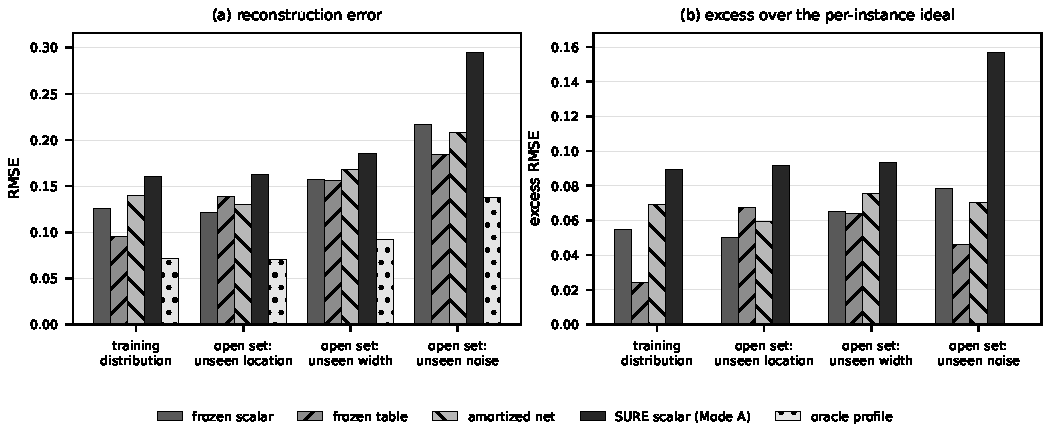
\includegraphics[width=\linewidth]{figures/probe.pdf}
\caption{A minimal empirical probe of the risk gap on a constructed open inversion task, reproduced by \texttt{experiments/probe.py}. Panel (a) reports the reconstruction error of each rule and panel (b) its excess over the per-position ideal of the instance. The corpus-fitted table is the best rule on the training distribution and the only rule within a third of the ideal, and its excess grows by a factor of $1.9$ to $2.8$ on the open set while the ideal is unchanged. Per-instance SURE, the evidence-instantiated rule of the analytic path, and the amortized map do not close the headroom, which is the cost side recorded in Section~\ref{sec:cost}.}
\label{fig:probe}
\end{figure}

\subsection{Relation to Uncertainty Quantification}

Bayesian deep learning distinguishes two kinds of uncertainty: data uncertainty comes from observation noise, and epistemic uncertainty comes from ignorance of model parameters, the latter decreasing as training data grows \citep{kendall2017}. This distinction happens to illuminate the decision axis brightly. Epistemic uncertainty is the statistical representation of Mode B's source of values: parameters are uncertain because their values are determined by a finite corpus, and a different sampling of the corpus gives different values. Mode A rules have no such degree of freedom; camera intrinsics do not change because a thousand more images are captured. Epistemic uncertainty can be calibrated well on closed benchmarks, but the calibrated benchmark itself remains in-distribution, and on the open set there is no distribution to calibrate against.

\subsection{Clues to Endogenous Mechanisms}

Mode A is not an invention of this paper; it has long-standing counterparts in neuroscience. Predictive coding theories of the visual cortex hold that higher levels keep sending predictions of the input to lower levels, which only pass back prediction errors \citep{rao1999}; the free-energy principle describes perception as a whole as the inversion of a generative model \citep{friston2009,friston2010}, with systematic tutorials on its implementation details \citep{bogacz2017}. The common form of these theories is exactly Paradigm I: context rules are endogenous to a single generative objective, and the values of predictions are computed online from current evidence rather than looked up from a frozen parameter table. This paper does not claim that these theories can be copied directly into engineering; it points out only one thing: the inference architecture selected by natural evolution falls on the Mode A side of the decision axis, which is consistent in direction with the negation conclusion of this paper.

\subsection{Existence and Cost of Mode A}
\label{sec:cost}

Whether Mode A really exists determines the practical reading of this paper's conclusion. Existence is substantiated along two paths. The first is the analytic-invariant path: calibrated intrinsics, geometric computations, and coupling strengths solved online from current observations have values given directly by evidence and calibration, bypassing the corpus. The second is the per-instance optimization path: test-time optimization and online inversion solve the rule values separately for each input \citep{sun2020}, and transductive learning is its precedent under near-distribution conditions \citep{vapnik1995}. Predictive coding provides a third clue, already seen in the previous section. Within the range where Assumption A0 holds, Mode A is therefore not an empty class, and the practical reading of this paper's falsification is: a fixed-memory component alone cannot be complete, and a combination with Mode A mechanisms can be complete. On tasks where A0 fails, no mechanism is complete, but they remain within the reach of the negation: Mode B fails there too, except that no Mode A mechanism can take over either.

The cost must be stated plainly. The cost of the analytic-invariant path is constant to linear and negligible. The cost of the per-instance optimization path is about $10^2$ to $10^3$ times one forward computation and is the main bottleneck of real-time systems. The iterative inference path lies in between, depending on the number of iterations needed for convergence. The temptation of Mode B comes exactly from this cost difference: replacing one optimization with one forward pass. The engineering motivation for composite systems lies here too: use Mode B in cost-sensitive and in-distribution stages, and use Mode A in the critical stage of rule generation.

\subsection{Correspondence with Adaptive Control and Online Optimization}

The decision axis has a parallel in control theory. Gain-scheduled control requires the scheduling variables to be measurable and exogenous, with controller parameters looked up or computed from the current operating condition; this is exactly the control-theoretic form of ``rule values instantiated by current evidence'' \citep{shamma1990}; auto-tuning and model-reference adaptive control go further, letting the control law be generated online \citep{astrom1995}. Conversely, an offline-tuned fixed gain table is the control-theoretic embodiment of Mode B, and gain scheduling working by a fixed schedule table is exactly the control-theoretic version of the ``move one level up'' mechanism of the reach section: the schedule table itself is still given by offline experience. Algorithms in online convex optimization that update decisions along the current loss sequence likewise belong to the Mode A side \citep{hazan2016}. The difference is equally worth writing down: online tuning of control laws is guaranteed by Lyapunov stability theory, whereas the correctness of Mode A inference currently has no corresponding stability theory; this is an open problem and the main theoretical gap in the engineering of Mode A.

\subsection{Abstention and the Composite Path}

Two alternative paths need a direct response. The first is detect-and-abstain: the component is highly accurate in-distribution, and it detects anomalies out-of-distribution and refuses to answer. An abstention mechanism decomposes the task into answering and refusing, but completeness requires correct answers on all inputs, and an abstaining system still faces the same decision axis on the inputs it does not refuse; if the refusal rule itself is carried by fixed parameters, detection fails on the open set as well, and the known difficulties of out-of-distribution detection are documented in the literature \citep{hendrycks2016}. Abstention therefore does not escape the decision axis; it merely moves the failure from the answering stage to the detection stage. Abstention is not a dead end: when the refusal criterion is instantiated by evidence, the system can fall back to a search path guided by the measurement model, confining the failure to the detection stage.

The second is composite systems: fixed-memory components propose candidates and likelihoods, Mode A mechanisms generate rules from current evidence, and the arbitration stage controls complexity on near-tree substructures. The limitations section gives necessary-condition-level guidance for composite systems, and one positive sentence is added here: in the legitimate form of a composite system, the credit for completeness goes to the Mode A mechanism, and the Mode B components in it still earn their keep, which is consistent with this paper's delimitation of the weak claim. This also answers the question that engineering practitioners care most about: existing end-to-end systems remain legitimate in-distribution, and what needs to be added is the Mode A loop of rule generation.

\subsection{Design Implications}

Rewrite the decision axis as three engineering questions for system design. First, where do the rule's values come from: corpus statistics, manual setting, current evidence, or analytic calibration. Second, are these values frozen at inference time: frozen is Mode B, and online instantiation is Mode A. Third, on the open set, who is responsible for instantiating the rule: if no mechanism is responsible, the system does not possess completeness for open inversion tasks. The minimal legitimate composite form is therefore: Mode B components provide candidates and likelihoods, a Mode A mechanism generates the rules, and the arbitration stage runs on near-tree substructures. The three questions correspond respectively to the operational readings of Definition~3, Proposition 4, and Theorem 5; the reverse direction, deciding the mode of an implementation that already exists, is the procedure of Section~\ref{sec:procedure}.

\subsection{Limitations}

This paper has four limitations. First, the satisfiability of Criterion P4 is a load-bearing empirical question, and Section~\ref{sec:p4} states the criterion in two components: tasks whose demand can be exactly identified from a fixed corpus fail the barrier condition, and tasks whose fine-scale demand reversals are rare fail the realization condition. In both cases the task is outside the class and a fixed-memory component can be complete, the linear-demand example of Section~\ref{ch:intro} marking the first boundary. No magnitude claim is made: what the barrier-to-gap proposition gives is the floor $\kappa$ of \eqref{eq:floor}, a positive constant attached to the task rather than an unbounded gap. The positive claims additionally need Assumption A0, and tasks whose demand depends on unobserved structure with no trace in the evidence do not satisfy A0, so no mechanism is complete there. Second, the falsification targets ``solo use is complete''; for composite systems it gives only necessary-condition-level guidance and design implications: any fixed-memory component appearing in a combination still has its rules in Mode B, and for a composite system to be complete, some other Mode A mechanism must be present, but this paper gives no sufficient conditions for composite systems. Third, the machine verification covers the carrier-independent algebraic core and the structured general forms, and the remaining modeling components are only the four items listed explicitly in Section~\ref{ch:verify}. Fourth, on the concrete implementation of Mode A, namely how to engineer context rules to be instantiated on the spot by current evidence, this paper gives existence paths and cost magnitudes but no construction scheme; this is the direction of future work. Empirical quantification likewise belongs to future work, with the probe of Section~\ref{sec:probe} standing as a first measurement on a constructed task: what remains is the same comparison of fixed, amortized, and per-instance rule families on a standardized benchmark such as \citep{leuschner2021}, contrasted with data-consistent frozen baselines, together with estimating the barrier separation and the realization level of a concrete task; this paper makes no experimental commitment about the open set of a real deployment.

\section{Conclusion}
\label{ch:conclusion}

To sum up, what this paper proves is: once the values of context rules are solidified by a corpus and frozen at inference time, no fixed-memory component, whether in the form of a neural network or a Bayesian network, possesses the completeness to independently complete open inversion tasks, and the two theorems share one and the same kernel. The argument unfolds along a decision axis: ill-posedness forces inference to use context, Lemma 1 excludes the global scalar from realizing a heterogeneous profile, Lemma 2 excludes frozen extrinsic coefficients from realizing a heterogeneous profile and converges the criterion onto the source, Criterion P4 and Lemma 3 require values to be instantiated by current evidence, Propositions 4 and 6 complete the classification, and Theorems 5 and 7 close the case. An equivalent, more prudent phrasing holds as well: no frozen rule family can be uniformly optimal on the open set; a frozen family offers at most in-distribution guarantees or guarantees vetted by analytic data consistency, while worst-case guarantees in the pointwise or expected sense require evidence instantiation. The relation to the existing literature has been clarified: the amortization gap records the empirical form of the Mode B gap, No-Free-Lunch gives the algorithm-level universal negation, and this paper fills in the component-level completeness negation between the two and gives a unified decision axis; in relation to No-Free-Lunch, this paper is an instantiation of its converse on the class of open inversion tasks.

This reach is not limited to the two kinds of networks: Markov random fields, conditional random fields, Gaussian mixture models, dictionary learning, kernel methods, and other components, as long as their context rules are carried by parameters trained offline or set by hand, all belong to Mode B and fall within the same falsification; random-field implementations whose coupling strengths are computed online from current evidence belong to Mode A and are outside the negation. The boundary of the conclusion is equally sharp: tasks whose demand can be exactly identified from a fixed corpus are outside the class, and there a fixed-memory component can be complete; the falsification stops exactly where the demand becomes freezable. The exclusion itself is not tied to the quadratic smoothing form of that classical problem: Lemma 1 is proved for a separable data term with an arbitrary even differentiable pairwise potential and without convexity, and its minimal obstruction is an equivalence rather than a sufficient condition, namely one single position whose required strength ratio changes between two admissible configurations. That condition excludes every frozen coefficient family, however many entries the table has; the global scalar is the case in which the ratio must also be common to all positions, which is why the scalar is the shallowest member of the excluded class rather than a special case to be defended separately. For Bayesian networks, beyond the negation there are two further walls of different status: the absence of a perceptual proposal layer, which is the negation read at the input interface rather than an independent theorem, and treewidth blow-up when the source of structure is missing, which is an external hardness result orthogonal to the negation.

Negation is not disparagement: the achievements of these components on closed benchmarks are genuine, and what this paper negates is only the universal claim ``solo use is complete'', not the usefulness of these components in combinations. The algebraic skeleton of the argument chain has been machine-verified with Lean 4 and Mathlib, with zero \texttt{sorry} and zero warnings. The other side of the decision axis, namely the engineering implementation of Mode A, is left to future work.


% JMLR requires an Acknowledgements and Disclosure of Funding section,
% placed before the appendices and the references. It must declare both
% (i) financial activities supporting the work and (ii) competing
% interests outside the submitted work.
%
% The author has confirmed that this work received no specific funding,
% so the funding declaration below is final (no placeholder remains).
\acks{The Lean~4 development reported in Section~\ref{ch:verify} was carried out with the Lean~4 proof assistant and its mathematical library Mathlib; the author thanks the Mathlib community for maintaining it. The verified artifact described in Section~\ref{ch:verify} is distributed in the \texttt{lean-proof} directory of the paper's repository, together with the \texttt{lean-toolchain} file that pins the toolchain version.

Funding: this research received no specific funding.

Competing interests: the author declares no competing interests.}

\vskip 0.2in
\bibliography{reference}

% The artifact index (layout, reproduction, axiom budget, the map from paper
% items to Lean declarations, and the premise lists of the load-bearing
% declarations) is published as the separately hosted online appendix, built
% from online-appendix/ by  ./build.sh appendix . It is deliberately kept out
% of this file: appendix pages count toward the JMLR page limit, and the paper
% points to the online appendix from its verification section instead.

\end{document}
